%Article
\documentclass[10pt]{report}

%appendix
\usepackage[toc,page]{appendix}

\DeclareUnicodeCharacter{2212}{-}

%Feyn
\usepackage{scalerel}
\newcommand{\mylbrace}[2]{\vspace{#2pt}\hspace{6pt}\scaleleftright[\dimexpr5pt+#1\dimexpr0.06pt]{\lbrace}{\rule[\dimexpr2pt-#1\dimexpr0.5pt]{-4pt}{#1pt}}{.}}
\newcommand{\myrbrace}[2]{\vspace{#2pt}\scaleleftright[\dimexpr5pt+#1\dimexpr0.06pt]{.}{\rule[\dimexpr2pt-#1\dimexpr0.5pt]{-4pt}{#1pt}}{\rbrace}\hspace{6pt}}

\begin{filecontents*}{vovalblob.mp}
vardef vovalblob (expr bd, a) (text vl)=
  forsuffixes $=vl:
    if not vexists $: venter $; fi
    vlist[vlookup $]decor.shape := fullcircle xscaled a;
    vlist[vlookup $]decor.size := bd;
    vlist[vlookup $]decor.sty := "shaded";
 endfor
enddef;
\end{filecontents*}
\def\fmfovalblob#1#2#3{\fmfcmd{input vovalblob; vovalblob ((#1), (#2), \fmfpfx{#3});}}


%Standard thesis size
\usepackage[a4paper,left=3cm,right=2.5cm,top=3cm,bottom=3cm,]{geometry}

%\usepackage{metafont}
%\usepackage{feynmf}
%\usepackage{feynmp}
\usepackage{feynmp-auto}

%comment large sections of text. 
\usepackage{comment}
% \begin{comment} 
% Commented text 
% \end{comment} 

%To make [H] Work
\usepackage{float}

%Loading comment package 
\usepackage{comment}

% for fancy looking tables
\usepackage{booktabs}   

%This package slashes dirac operators 
\usepackage{slashed}

% Good old Checkmarks
\usepackage{pifont}

%Not sure
\usepackage[english]{babel}

% References I'd guess 
\usepackage{hyperref} 
%\usepackage{apacite} 

%Mathematical expressions 
\usepackage{amsmath}
\usepackage{amssymb}

% Where are the images
\usepackage{graphicx}
\graphicspath{{./Images/}}

% inputs 
\usepackage[utf8]{inputenc}

%Using Sub files
%Perfect comment Pedro, cat --> this says cat
\usepackage{subfiles}

%images in here 
\graphicspath{{./Images/}}

%Horizontal line
\usepackage{cancel}

%tables 
\usepackage{tabularx}

%using a colored text 
\usepackage{xcolor}

\newcommand{\ro}[1]{\textrm{#1}}
\newcommand{\U}[1]{\mathrm{U}(1)_{\mathrm{#1}}}
\newcommand{\Z}[1]{\mathrm{Z}(1)_{\mathrm{#1}}}			
\newcommand{\SU}[1]{\mathrm{SU}(2)_{\mathrm{#1}}}			

% Thesis format
\usepackage[DF,newLogo]{uaThesis}
\setlength\extrarowheight{2pt}
	
% optional: visual delimiters for floats (figures and tables)
\def\topfigrule{\kern 7.8pt \hrule width\textwidth\kern -8.2pt\relax}
\def\dblfigrule{\kern 7.8pt \hrule width\textwidth\kern -8.2pt\relax}
\def\botfigrule{\kern -7.8pt \hrule width\textwidth\kern 8.2pt\relax}

%nova pagina ao fim da seção
\usepackage{titlesec}
\newcommand{\sectionbreak}{\clearpage}

%\renewcommand{\cftsecfont}{\rmfamily\mdseries\upshape}
%\renewcommand{\cftsecpagefont}{\rmfamily\mdseries\upshape} % No bold 
%\usepackage{apacite}
\def\ThesisYear{2020}

% Added in November 
\usepackage{flexisym} % This package allows me to use a Prime in text format 

%Shamelessly stolen, this makes life so much easier 
\renewcommand{\(}{\left(}

\renewcommand{\)}{\right)}

\renewcommand{\[}{\left[}

\renewcommand{\]}{\right]}

\newcommand{\del}{\partial}

%check marks
\newcommand{\cmark}{\ding{51}}%
\newcommand{\xmark}{\ding{55}}%

\begin{document}


\TitlePage
  \HEADER{\BAR\FIG{
\includegraphics[height=60mm]{uaLogoNew.pdf}}} 
%	
  {\ThesisYear}
  \TITLE{João Pedro \\ Dias Rodrigues }
        {A study of possible beyond the standard model frameworks containing multiple scalars and their implications in the search for new physics. \\ \ \\ Um estudo de modelos numa arquitetura para além do modelo padrão e o seu possível impacto em nova física}
\EndTitlePage
\titlepage\ \endtitlepage % empty page

\TitlePage
  \vspace*{55mm}
  \TEXT{\textbf{o j\'uri~/~the jury\newline}}
       {}
  \TEXT{presidente}
       {\textbf{Margarida Facão}\newline {\small
        Professora Auxiliar do Departamento de Física da Universidade de Aveiro}}
  \vspace*{5mm}
  \TEXT{vogais}
       {\textbf{António Morais}\newline {\small Investigador Nível 1 do Departamento de Física da Universidade de Aveiro}}
  \vspace*{5mm}
  \TEXT{}
       {\textbf{Nuno Castro}\newline {\small
        Professor Assistente da University of Minho. }}
  \vspace*{5mm}
\EndTitlePage
\titlepage\ \endtitlepage % empty page

\TitlePage
  \vspace*{55mm}
  \TEXT{\textbf{agradecimentos~/\newline acknowledgements}}
       {Honestamente acho que isto vai ter que ser escrito antes da entrega,{\color{red} REMINDER agradecer ao Morais! Pedro Ferreira Roman e Ian, sem o trabalho deles estava perdido. }}
  \TEXT{}
       {Honestly this will be written in english translated poorly from above :) }
\EndTitlePage
\titlepage\ \endtitlepage % empty page

\TitlePage
  \vspace*{55mm}
  \TEXT{\textbf{Resumo}}
       {O Modelo Padrão é neste momento o paradigma na analise de física de particulas, este une numa arquitectura autoconsistente e propriamente motivada três das quatro forças fundamentais do universo, no entanto, o consenso cientifico é que modelo padrão esta incompleto, visto que apesar do excelente acordo entre muitas das suas previsões e a realidade, imensas experiencias estão a mostrar fenómenos que o modelo padrão não consegue reconsiliar. 
\\ \ \\ 
Devido a estas falhas, estão cada vez mais a ser propostos modelos motivados por objectivos, como a inclusão de grande unificação ou a previsão de materia escura, para tentar completar ou substituir o modelo padrão. \\
\ \\
Neste trabalho começamos por uma breve revisão do Modelo Padrão, e de seguida apresentamos dois modelos que se intintulam para alem do modelo padrão com o objectivo de os introduzir toericamente como contexto para a apresentação de uma analise numerica sobre os possíveis sinais de nova física que cada senario podera trazer.  
       }
\EndTitlePage
\titlepage\ \endtitlepage % empty page

\TitlePage
  \vspace*{55mm}
  \TEXT{\textbf{Abstract}}
       {
       This part will be in English. Translated from above. 
       }
\EndTitlePage
\titlepage\ \endtitlepage % empty page


\pagenumbering{roman}
\tableofcontents

\cleardoublepage
\listoffigures

\cleardoublepage
\listoftables

\cleardoublepage

\pagenumbering{arabic}
\setcounter{page}{1}

%\section{Labels}

%{{\color{green}A paragraph or text to be added later  }

%{{\color{red}   A mistake or a question that is likely wrong }

%{{\color{blue}  A comment or doubt to ask or check}

%{{\color{gray} Excess? Probably will cut, waiting for advice} 

%\chapter{Introduction}
%\label{ch:Intro}

\newpage

\chapter{Introduction}
\label{Chap:Introduction}
%\section{Introduction}

%\section{The Sturdy SM with some holes}

% The modern study of particle physics must be taught trough the Standard Model (SM) of particle physics. 
Our current understanding of all subatomic phenomena must be understood trough the Standard Model (SM) of particle physics. 
%
% The SM has thus far been the best descriptor for the experimentally observed spectra of particles and their interactions at all current probable scales. 
%
The SM has thus far been the best descriptor for the experimentally observed spectra of particles and their interactions at the electroweak (EW) scale. 
%
Being that, finally, in 2012 a resonance was discovered at the Large Hadron Collider (LHC) that confirms the existence of its last predicted particle, the Higgs boson, finally revealing all of the models particles and proving the existence of the Higgs mechanism \cite{collaborations2016measurements}. 
% Old Citations
%\cite{Aad_2012,chatrchyan2012observation,collaborations2015combined,collaborations2016measurements}

The development of the SM was a arduous task, leading scientists successfully combine three of the four fundamental interactions of nature, the electromagnetic, weak and strong interactions, in a well motivated framework. 

However, despite its successes the SM still lacks a strong explanation for several experimental observations. 
%
%They have become more numerous by the decade and to provide a "short" overview of some of them. 
%
To enumerate some of these previously alluded too problems, we have:
%
First, we have the fact that the SM can not account for one of the most important cosmological discoveries of the century, the existence of dark matter \cite{Bergstr_m_2000}. 
%
This is a fundamental flaw since the SM lacks a possible dark matter candidate, or dark particle. % {\color{red} (It is already discussed in 6. Should I put the ciation here again?).} 
%
%Secondly, neither the SM, nor the theory of general relativity, offer any justification for the existence of baryon asymmetry in the universe, i.e. why is the universe primarily made of matter rather than anti-matter \cite{book_Baryion}. 

Secondly, the SM does not offer any justification for the existence of baryon asymmetry in the universe, i.e. why is the observable universe primarily composed of matter rather than anti-matter \cite{book_Baryion}. 
%
%Note, that a popular proposed scenario as to explain cosmic baryon asymmetry is the Electroweak baryogenesis (EWBG) which requires some sort of new physics (NP) structure \cite{Morrissey2012}. 

Thirdly, the SM suffers from peculiar oddities in the fermion sector in the form of unjustified mass and mixing hierarchies. This is usually refereed to as the flavor problem and is considered a sizable drawback of the SM. 
%
As an example, we observe the top quark mass ($\mathcal{O}(100)$ GeV) to be five order of magnitudes heavier than the up quark ($\mathcal{O}(1)$ MeV), and eleven orders of magnitude above the highest neutrino mass limit ($\mathcal{O}(1)$ eV) set by kinetic beta decay analysis \cite{Mertens_2016}.
%
%{ ( \color{red} Ask Morais: Eu sei que existem experiencias de oscilações mas eu acho que só havia um higher limits de massa nos neutrinos. Basicamente eu não sei se dizer massas de neutrinos é correto. ) }
%
These high differences are thought to be too large to be natural, so a physical property that would justify such gap is a desired characteristic of many Beyond the Standard Model (BSM) frameworks. 

Fourth, neutrino masses (as alluded to) are not included in the SM. Although there are precise oscillation measurements that measure masses differences in the eV range with precise mixing in between 3 different generations of neutrinos \cite{PhysRevD.89.013001}. 

In addition to these, there are still many other subtitle flaws, like the lack of a strong phase transition, the $R_{\kappa}$ parameter and $g-2$ anomaly of lepton magnetic moments, etc. 
%
These are just some of the typical justifications given to explore possible BSM scenarios. 
%
The holy grail of which would be a model that solves all these problems in a properly motivated framework that addresses these and many more cosmological and phenomenological problems and is in harmony with all measurements.  

For now such a model remains far out of reach, and given the large number of possible solutions, the narrowing down of theories through phenomenological studies is a very worthwhile endeavor. This work will be a review of two such studies. % We try to present one of these studies in this work. % to the steady advancement of a more complete theory. 

The ``normal" procedure for these kinds of studies consist in performing large a numerical analysis of all possible combinations of free parameters of a given model, which we call the parameter space, as to narrow it down trough compassion with modern bounds set by experiments. This allows us to predict exactly what observations this model could still allow for in experimental detection and measure if the proposed model could have a significant impact as to explain observed deviations or if it is, in a extreme case, completely excluded by modern limits.   
%
% and see how much phenomenology it can explain, or not, and even perhaps exclude the model under modern collider experiments.

Paradoxically, as of late these studies have become progressively harder to perform regardless of the improvement in hardware given that the available space for NP gets reduced by each successful particle experiment. 
%
Chief among them are the ATLAS, CMS experiments at the LHC, whose large amount of collect data over past years is setting ever more stringent bounds on viable parameter spaces of popular BSM scenarios. 
%
And as available space for new physics decreases, it becomes more challenging to reveal remaining space without falling within the possibility of fine tuning our model. Fine tuning consists in carefully balancing several contributions as to, cancel or magnify as to be allowed by current bounds.    

%{\color{blue} How to properly explain what fine tunning is? Should I?}

Note, that the SM has shown itself consistence with most constraints that were initial believed to be a possible gateway to NP i.e. divergences from its predictions. Thus, the search continues for hints at possible directions to complete the SM. One of these is brought to use trough flavor physics, as we'll soon examine further on. 

Conventionally, phenomenological simulations of BSM searches in these multi-dimensional parameter spaces have been made in large computer-clusters requiring several weeks of computational time trough simple Monte-Carlo methods. 
%
These simple methods are the basis for the work presented in this thesis although some modern studies have incorporated new methods to scan these complex problems like machine learning. Similar to done by our colleagues in \cite{freitas2020phenomenology}. These new methods promise to greatly increase the efficacy of similar studies.  
%
%Although this is the basis of the work presented here a effort was made to incorporate new machine learning routines via the initial building of smaller learning sets by conventional methods. 
%
%Unfortunately this wasn't accomplished in this work due to the expectational setbacks. A feature of this year, that affected partially the quality of the work. 

%%%% so far so good

%During this thesis we embark in a small expedition into two possible BSM scenarios.

Over the course of this thesis we intent to perform two of these BSM studies. However we must begin by laying down the fundamental basis for this type discussion by presenting a short overview of the SM. 
%
%In this thesis we will embark in two of these kind of BSM studies.  
%
%Start by laying down the fundamental basis for this BSM discussion by presenting a short overview of the SM followed by a discussion into potential extensions of this framework.
Afterwords we will present, first the B-L-SM (Baryon-Lepton-SM) model, a simple unitary extension of the SM - and then, move on to a more complex model with additional Higgs doublets fields as an attempt to present a framework that addresses the flavor problem via the Three Higgs Doublet Model (3HDM) with a stabilizing symmetry.
%
We will see how each of these models addresses specific problems differently and discuss the advantages and disadvantages of a simple unitary extension versus a multiple doublet approach. 

For example multiple Higgs doublets can easily offer an explanation for the observed excess of charge parity or $\mathcal{CP}$ violation but suffer from the possible inclusion of tree-level Flavour Changing Neutral Currents (FCNCs). 
%
These FCNCs are undesirable \cite{ILYUSHIN2020114921}, at least in large number, given current observations, so mechanisms have to be put in place to prevent them, while in the case of the simple unitary extensions such problems tend to not arise \cite{Huitu2019}. 

We also want to stress that, while the minimal structure of the Higgs sector postulated by the SM is not an immediate contradiction to experimental measurements it is not manifestly required by the data. 
%
In fact, an extended scalar sector is often desirable feature of BSM scenarios despite the tight bounds on Higgs boson couplings to the SM gauge bosons and heavy fermions. 
{\color{red} Ask:Morais How do I cite https://pdg.lbl.gov/2019/reviews/rpp2018-rev-higgs-boson.pdf exactly instead of the whole corpus}.   

These additions are partially motivated by the fact that in the SM, the single Higgs doublet is a bit "overstretched" in the SM.
%
It  takes  care,  simultaneously of the gauge boson masses, up and down-type quarks masses and leptons masses. 
%
N-Higgs-doublet models have multiple scalar and complex fields that can relax this, while the simpler unitary additions cannot address this observation % {\color{red} Is it true? Couldn't we have a singlet generate the top quark masses or only the third generation, do I need a citation?}.   
%
In fact these multiple Higgs doublet models are often engineered based on a naturalness argument, that is,  the  notion  of  generations  can  be  brought  to  the  Higgs  sector and these might help explain mass hierarchies. % This is not the particular case of the model we will present in this thesis. 

%Both these extensions have the bonus of leading to remarkably rich  phenomenology (for a detailed review, see e.g. Refs. ( \cite{branco1999cp,Branco_2012,Ivanov_2017} ). And in general BSM scenarios offer features  as  several  Higgs  bosons,  charged  and neutral, modification of the SM-like Higgs couplings, FCNC at tree level, additional forms of CP-violation from the scalar sector, and opportunities for cosmology such as scalar DM candidates and modification of the phase transitions in early Universe. {\color{blue} Repeated, Fix later.} Also, many BSM models including supersymmetry (SUSY), gauge unification models, and even string theory constructions naturally lead to several Higgs doublets at the electroweak scale.

%We give a higher repute to the Higgs Sector since fermion masses and mixing patterns relate often to the specific structure of the Higgs sector. Also, the addition of new scalars offer a large playground for collider experimentation and often offer the inclusion of new neutrino physics. 

%In short two particular multi-Higgs models will be presented in this work a phenomenological study of a 3 Higgs Doublet model (3HDM) with softly broken $\U \times \mathrm{Z_2}$ symmetry and a simple Unitarity, $\mathrm{U(1)}$, extension of the SM based on the apparent Baryon minus Lepton symmetry (B-L-SM). We'll investigate what can be learned from these models and what other physical experiments constrict them. 

%The SM extensions featuring non-minimal Higgs sectors with extra Higgs doublets in analogy to fermion generations in the SM provide a fruitful playground for constructing successful BSM scenarios (for a detailed review, see e.g. Refs. \cite{branco1999cp,Branco_2012,Ivanov_2017} ).

%There is also no constraints stemming from the $\rho$ parameter here.  Since all doublets couple to the gauge-bosons in the same way, the W and Z masses are determined by the single value, the sum of real VEVs. Assuming this value is 246 GeV it would retain the condition $\rho = 1 $ at tree-level. 

%Multi-doublet models offer novel opportunities for CP-violation.  Within the SM, it is put by hand coming entirely from the Yukawa matrices which must be complex.  In multi-doublet models, a relative phase between vevs can arise just as a result of the minimization of the potential. Leading to a more natural and spontaneous CP-violation. 

%A real or even complex singlet extension is a also simple pathway to extending the SM. In a generic model with a SM Higgs Doublet the addition of a generic gauge singlet scalar, S, could prove a link between the SM fields and a unknown hidden sector. 
%
%In spite of our ignorance of this hidden sector, we can simply assume a generic renormalizable self-interaction for the scalar S and investigate the joint $(\phi,S)$ potential. This would lead to a generic mixing, $\alpha$ between scalars. 

%In the case the additional scalar field is complex this brings a additional degree of freedom and has the possibility of 3 neutral scalars mixing, depending on the shape of the VEV. Producing  a slightly  richer  collider  phenomenology  and  complicating its analysis.  

%Are heavily constricted from experimental measurements we know that in this framework fermions and gauge bosons should primary couple to $h_\phi$. This type of mixing suppression, ($\alpha < 10^3$), but even so the heavy Higgs can in most cases decay into a pair of light ones if this channel is open kinematically, providing a avenue for detection. 

%On the other hand, one or both new scalars can be symmetry protected against decay, yielding simple models of one or two-component dark matter or models with one DM candidate and a strong electroweak phase transition.

%Before moving on, let us make a remark on the (absence of) CP-violation in the singlet extension of SM. Although the potential contains many complex coefficients, it does not produce CP-violating effects in the scalar sector, see \cite{branco1999cp}.







\chapter{The Standard Model of Particle Physics}\label{chapter:StandardModel}
%\section{The Standard Model of Particle Physics}
%
%To pave the way for our future studies we present the SM. Complete with a overview of it's mechanisms and a brief historical introduction.
%

\Joao{Não é necessário fazer uma secção só para isto. Comentei section{Motivation}}
%\section{Motivation}

% { \color{red} Note! The motivation should explain why we are going indepth into flavour, and the Yukawa sector. There has to be a purpose to this section! } 

\Joaorep{Has}{As} stated \Joaoadd{in Chapter.~\ref{chapter:Introduction}}, it is hard to question the validity of the SM as a successful, at least approximate, framework with whom to describe the phenomenology of Particle Physics up to the largest energy scales probed by collider measurements so far\Joaoadd{. A}lthough\Joaoadd{,} some inconsistencies remain and must be addressed.  
%
The SM was proposed in the nineteen sixties by Glashow, Salam and Weinberg \Joao{Não é bem verdade, o SM é um conjunto de várias teorias (QCD + Higgs sector + Electrofraca). O que estes autores introduziram foi a teoria electrofraca. Acho que fica bem aqui por a referência dos papers deles.} and since \Joaoadd{then} it has been extensively tested. Both in contemporary direct searches for new physics and indirect probes via e.g. flavour anomalies and precise electroweak parameter measurements in proton-electron collisions. \Joao{Refs.} %, { \color{gray} and as said, it's been consistent with most to date.} 

The path to the formulation of the SM came from previous principles \Joaorep{relating}{related} to symmetries in nature, specifically symmetry in physical laws. 
%
In fact, much \Joaorep{in}{of} modern physics can be attributed to Emmy Noether's work. She deduced, trough her first theorem, that if the action in a system is invariant under some group of transformations (symmetry), then there exist one or more conserved quantities (constants of motion).\Joao{Ref.} \Joaoout{which are associated to these transformations.}

Physicist\Joaoadd{s} took this idea and were led to the fundamental question behind the SM, is it possible that upon imposing to a given Lagrangian the invariance under a certain group of symmetries to reach a given form for \Joaorep{it's}{its} the dynamics? 
%
These dynamics would be in our context, particle interactions. This train of thought first led to Quantum Electrodynamics (QED), then Quantum Chromodynamics (QCD) and finally the SM.  \Joao{Esta frase tem que ser reescrita. Eu sei o que queres disser, mas está um pouco confuso e difícil de ler. Também estás a combinar dinâmica e interacções, que são coisas distintas. Dinâmica corresponde a como os campos evoluem no espaço-tempo.}
%
We can quote Salam and Ward: % A. Salam and J. C. Ward, Nuovo Cim.19, 165 (1961). 

\textit{“Our basic postulate is that it should be possible to generate strong,  weak and electromagnetic  interaction terms (with all their correct symmetry properties and also with clues regarding their relative strengths) by making local gauge transformations on the kinetic energy terms in the free Lagrangian for all particles.”}
\Joao{Eu retirava a quote, ocupa espaço desnecessário, tendo em conta que apenas rearfima o que disseste anteriormente. E também é mais uma referência que ocupa espaço.}
We are glossing over a lot of complexity here, and for the SM to be properly formulated\Joaoadd{,} additional concepts \Joaorep{would be}{are} required. In the case of \Joaoadd{the} weak interactions, the presence of \Joaorep{very heavy}{massive} weak gauge bosons require the new concept of spontaneous breakdown of the gauge symmetry \Joaorep{and the}{via that is known as the} Higgs mechanism \cite{higgs1964broken,englert1964broken,guralnik1964global} \Joao{Podes tirar uma. Tens muitas referências, por isso temos de reduzir o espaço ocupado}. 
%
While the concept of asymptotic freedom played a crucial role \Joaorep{to describe perturbatively}{in describing} the strong interaction at short distances \cite{politzer1973reliable,gross1973ultraviolet} \Joao{Só uma ref.}.  

%\renewcommand{\cleardoublepage}{}
%\renewcommand{\clearpage}{}

\section{Internal symmetry of the Standard Model}\label{section:Symmetries_SM}
%
The SM is a \Joaoadd{gauge} \Joaoout{"standard"} \Joaoadd{Quantum Field Theory} \Joaoadd{(QFT)} \Joaoout{gauge theory}, that is \Joaoout{to say}, it is manifestly invariant under a set of field transformations. The SM gauge group, $\mathcal{G}_{SM}$, is seen in, \Joao{Aqui devias por uma referência ao SM, de um livro ou de lecture notes.}
%
\begin{equation}
\mathcal{G}_{SM} = \mathrm{SU}(3)_{\mathrm{C}} \times \SU{L} \times \U{Y}.
\label{eq:SM_Group}
\end{equation} 
%
\Joaorep{Here we have, first, the}{Where,} $\mathrm{SU}(3)_{\mathrm{C}}$\Joaoadd{, with C being colour,} \Joaoadd{is the} group \Joaorep{corresponding to}{that describes the} \Joaoout{quantum chromodynamics} QCD \Joaoadd{sector}, responsible for the strong force. \Joaoadd{T}his symmetry will remain unbroken by the electroweak \Joaoadd{vacuum expectation value} (VEV). Secondly, we have the $\SU{L} \times \U{Y}$ portion, \Joaoadd{with L being Left and Y the hypercharge},  that will be broken by the Higgs mechanism into $\U{Q}$, the electromagnetic gauge symmetry.
%
Each particle stems from a field that is charged in a particular manner on each of these groups. \Joaoout{, making the charge triplets we will come to later define.} 
%
Given the invariance under the group in Eq.\,\eqref{eq:SM_Group} \Joao{Vê no tex como é para fazer referências das equações}, it is impossible \Joaoadd{for} \Joaoout{have} any field \Joaorep{that is charged have a explicit mass term}{, besides the scalar field, to have an explicit mass term in the bare Lagrangian.}. This chapter will focus on how the mass of particles is generate \Joaoout{trough}{via} the Higgs mechanism. And offer a brief discussion of flavour physics in the SM and how flavour changing currents can point to \Joaoout{{\color{blue} New Physics (NP)}} \Joaoadd{NP}. 

%{ \color{gray} All masses for the fermions and leptons are generated trough their interactions with the Higgs Boson. This mass generation as the Higgs Boson settles into it's VEV is called the Higgs Mechanism. } 

\subsubsection{Gauge Group numbers}
\Joao{Subsubsections são um pouco desnecessárias na minha opinião, mas se quiseres podes deixar.}

The full set of quantum numbers \Joaorep{in all the SMs fields}{for the SM fields} are \Joaorep{described}{shown} in \Joaoout{the} \Joaoadd{T}ables \ref{table1} and \ref{table2}\Joaoout{, this is their color charge, weak isospin number and the hypercharge, written in that order as entries in each triplet.}
\\
\\
\Joao{Estás a confundir as coisas. A carga de cor e o número de isospin não é o que está na tabela. Para os grupos não abelianos, tu estás a indicar a \textbf{representação}. Por exemplo, quando disses, que o $A$ tem um número quântico de SU(2) de \textbf{3}, tu apenas estás a disser que ele é um tripleto de SU(2), $A^a=(A^1,A^2,A^3)$, sendo que o índice a está a correr sob a representação adjunta do grupo. Para campos com \textbf{2} eles são dobletos, para campos com \textbf{1} eles são singletos e portanto não participam na interacção. Por exemplo, o campo de Higgs é singleto de SU(3), logo não interage com os gluões.
A carga de cor é vermelha, verde ou azul e é propriedade dos quarks na interacção com os gluões (é uma espécie de carga eléctrica). O isospin fraco é definido como $I_w = Q - \frac{1}{2}Y$ com $Q$ a carga de partícula e $Y$ a hipercarga.}
%
\begin{table}[H]
\centering
\caption{Gauge and Scalar fields \Joaoout{dimensions} in the SM}
\label{table1}
\begin{tabular}{@{}cccccc@{}}
  \hline	
 Fields & Spin 0 field & Spin 1 Field & $\mathrm{SU(3)_C} \times \mathrm{SU(2)_L} \times \mathrm{U(1)_Y}$  \\
  \hline	
 Gluons  & $\times$  & $\Joaoadd{G}^{\Joaoadd{a}}$ & (\textbf{8},\textbf{1},0) \\	
A bosons & $\times$  & $A^{\Joaoadd{a}}$ & (\textbf{1},\textbf{3},0)   \\
B bosons & $\times$  & $B$ & (\textbf{1},\textbf{1},0)   \\
Higgs field & ($\phi^\pm, \phi^0 )$  & $\times$ & (\textbf{1},\textbf{2},1) \\ \hline
\end{tabular}
\end{table}
%
\begin{table}[H]
\centering
\caption{Fermion field \Joaoout{dimensions} in the SM}
\label{table2}
\begin{tabular}{@{}cccccc@{}}
  \hline	
 Fields & Spin $1/2$ Field & $\mathrm{SU(3)_C} \times \mathrm{SU(2)_L} \times \mathrm{U(1)_Y}$  \\
  \hline	
Quarks (3 gen.) & $Q=(u_L,d_L)$ & $(\textbf{3},\textbf{2},1/3)$ \\	
$\quad$        & $u_R$ & $(\textbf{3},\textbf{1},4/3)$   \\
$\quad$   & $d_R$ & $(\textbf{3},\textbf{1}, -2/3)$   \\
Leptons (3 gen.) & $L=(\nu_{e_L}, e_L )$ & $(\textbf{1},\textbf{2},-1)$  \\
$\quad$   & $e_R$ & $(\textbf{1},\textbf{1},-2)   $ \\ \hline
%
\end{tabular}
\end{table}
%
\Joao{Para grupos não abelianos, os números devem ser colocados a negrito. Também fiz umas pequenas alterações para ficar mais visível.}
From here, given the gauge group in Eq.\,\eqref{eq:SM_Group} and accounting for the charges and fields, we can derive the form of the SM's Lagrangian. These gauge groups are composed of 12 generators and are governed by the following algebra, 
% 
\begin{equation}
\Joaoadd{\left[ M_a , M_b \right] = i f_{abc} M_c} \quad \left[ T_a , T_b \right] =  \epsilon_{abc} T_c \quad \Joaoadd{\left[ M_a , T_b \right] = \left[ M_a , Y \right]} = \left[ T_b,Y \right] = 0 
\end{equation}
%
where for \Joaoout{the} $\mathrm{SU(3)_C}$ \Joaoout{triplets}, \Joaoadd{we have} $\Joaoadd{M_a}= \lambda_a/2$ \Joaoadd{with} $a = 1, . . . , 8$ \Joaoout{contrary to $\mathrm{SU(3)_c}$ singlets where, $L_a = 0$}, \Joaorep{As for the}{,for} $\mathrm{SU(2)_L}$ we have $T_i= \sigma_i/2 $ \Joaoadd{with} $i = 1, 2, 3$, \Joaoout{being that again for singlets $T_b=0$} \Joaoadd{and} $Y$ is the generator of $\mathrm{U(1)_Y}$. The symbols $\lambda$ and $\sigma$ represent the Gell-Mann and Pauli matrices, respectively. \Joao{Também estou a fazer alterações nas equações com verde. Em alguns casos é díficil de ver.}

\subsection{Fields, Particles and Lagrangian of the SM}

From these fields\Joaoadd{,} \Joaorep{the physical states of the SM, it's particle spectrum,}{the particle spectrum of SM} is composed by\Joaoout{, first,} the gauge bosons, \Joaoout{the weak force carriers,} $W^\pm$ and $Z$ \Joaoout{bosons}, \Joaoadd{mediators of the weak interaction} \Joaorep{and}{,} the photon $\gamma$, the electromagnetic interaction messenger and the strong force mediators, the gluons, $\Joaoadd{G}$, as well\Joaorep{, of course,}{as} \Joaoout{by} the matter particles, the fermions, composed by the quarks and leptons. \Joaoadd{A physical spin-0 scalar also emerges, known as the Higgs.}

Leptons and quarks are organized in three generations each, with 2 pairs by each generation leading to 6 different particles \Joaoout{for each}. 
%
For quarks we have the up and down for the first generation, charm and strange for the second as well as \Joaoadd{the} top and bottom for the third one. 
%
Similarly, there are 6 types of leptons, the charged ones, electron, muon and tau, and the associated neutrinos. These are represented in different manners, being that the quarks are represented by the letters $(u,d,c,s,t,b)$ while leptons as $(e,\nu_{e},\mu,\nu_{\mu},\tau,\nu_{\tau})$. 

Fermions are half integer spin particles\Joaoadd{,} half of which have electrical charge (except the neutrinos).  While quarks interact via the weak, electromagnetic and strong forces, the charged leptons only feel the electromagnetic and weak forces and the neutrinos are weakly interacting.  
%
A physical fermion is composed of a left-handed and a right-handed field. \Joaorep{While the left \Joaoadd{components} transform as $\mathrm{SU(2)_L}$ doublet}{The left-handed components of the fermions are doublets under $\mathrm{SU(2)_L}$} and can be written as
%
\begin{equation}\label{eq:Left_boys}
L^i= \begin{pmatrix}
\nu_{e_L} \\ e_L 
\end{pmatrix},
\begin{pmatrix}
\nu_{\mu_L} \\ \mu_L 
\end{pmatrix},
\begin{pmatrix}
\nu_{\tau_L} \\ \tau_L 
\end{pmatrix} 
\quad 
\text{and} \quad Q^i= \begin{pmatrix}
u_{L} \\
d_L 
\end{pmatrix},\begin{pmatrix}
c_{L} \\
s_L 
\end{pmatrix}
,\begin{pmatrix}
t_{L} \\
b_L 
\end{pmatrix} \quad ,
\end{equation}
where the $i$ index stands for generation, often designed as the flavour index. \Joaorep{the latter are $\SU{L}$ singlets and can be simply represented as}{Conversely, the right-handed components are singlets of $\mathrm{SU(2)_L}$ and are represented as}
%
 \begin{equation}\label{eq:Right_boys}
e^i_R=\{e_R,\mu_R,\tau_R\}, \quad  u^i_R=\{u_R,c_R,t_R\}, \quad d^i_R=\Joaoadd{\{d_{R},s_{R},b_{R}\}}, 
\end{equation}
%
note also that the quarks form triplets of $\mathrm{SU(3)_C}$ whereas leptons are colour singlets \Joaoadd{meaning that only quarks interact strongly.} The Higgs boson also emerges from an $\mathrm{SU(2)_L}$ doublet with the form,
%
\begin{equation}\label{eq:Higgs_doublet}
H=\begin{pmatrix}
\phi^1 + \; i \; \phi^2 \\
\phi^3 + \; i \; \phi^4  
\end{pmatrix}, 
\end{equation}
%
\Joao{Não ponhas quad depois das equações. Tens que pensar que as equações são uma continuação do texto, e as vírgulas estão agarradas a letra anterior}
%The Lagrangian that describes all vector particles and gauge fields in the SM can be writen as
%
\Joaorep{Here}{where} we see the four components that correspond to the respective degrees of freedom of the Higgs Field.
% 
After the process of \Joaoadd{spontaneous symmetry breaking} (SSB) of the $\mathrm{SU(2)_L} \times \U{Y}$ group the charges \Joaoout{of the fermions along their QCD and QED numbers} become 
%
\begin{table}[H]\label{tab:Charges_post_SSB}
\caption{Quark and Lepton charges. \Joao{Novamente, a negrito para não abelianos}}
\centering
\begin{tabular}{ccc}
  \hline & $\mathrm{SU(3)_C}$ & $\mathrm{U(1)_Q}$ \\
  \hline 
Up type quarks $(u,c,t)$ & \textbf{3} & 2/3 \\
Down type quarks $(d,s,b)$ & \textbf{3} & -1/3 \\
Charged leptons $(e,\mu,\tau)$ & \textbf{1} & -1 \\
Neutrinos  $(\nu_e,\nu_\mu,\nu_\tau)$  & \textbf{1} & 0 \\
  \hline	
\end{tabular}
\end{table}

\subsubsection{Lagrangian formulation }
%
Given the SM gauge groups, \Joaoadd{seen in Eq.\,\eqref{eq:SM_Group}} and charges, \Joaoadd{seen in Tables \ref{table1} and \ref{table2}} the covariant derivative, $D_\mu$, \Joaoout{will} read\Joaoadd{s} as
%
\begin{equation}
\label{eq:PartialDefSM}
D_\mu = \partial_\mu - i \Joaoadd{g_s} \Joaoadd{M^a} G^a_\mu - i g T^i A^i_\mu - i g' Y B_\mu.
\end{equation}  
%
\Joao{Acho que o último tem de estar a dividir por dois. Confirma.} We can expect 3 different type of couplings, $g_s$ related to the $\mathrm{SU(3)_C}$ subgroup, $g$ to the $\mathrm{SU(2)_L}$ and $g^\prime$ to $\mathrm{U(\Joaoadd{1})_Y}$. The associated canonical field strength tensors would be,
\begin{equation}\label{eq:Field_strength_tensors}
\begin{aligned}
G_a^{\mu \nu} & = \partial^\mu G^\nu_a - \partial^{\Joaoadd{\nu}} G^\mu_a - g_s f_{abc} G_{\Joaoadd{b}}^\mu G_{\Joaoadd{c}}^\nu,  \\ 
A_a^{\mu \nu} & = \partial^\mu A^\nu_a - \partial^\nu A^\mu_a  - g \epsilon_{abc} A^\mu_b A^\nu_c, \\
B^{\mu \nu}   & = \partial^\mu B^\nu - \partial^\nu B^\mu.
\end{aligned}
\end{equation}
It is often convenient to present the SM Lagrangian in portions, usually divided in three sections\footnote{\Joaoadd{Of course, there is also the need for the introduction of gauge fixing terms and ghosts. However, this is merely a formal requirement and does not imply addition of new physical states.}},
\begin{equation}\label{eq:SM_baby_lagrangian}
\mathcal{L}_{SM} = \mathcal{L}_{kin}  +  \mathcal{L}_{Yuk} +  \mathcal{L}_{\phi}\Joaoadd{,}
\end{equation}
\Joaoadd{w}here we have the kinetic portion of the SM terms, $\mathcal{L}_{kin}$, responsible for  free propagation of particles, the Yukawa portion, $\mathcal{L}_{Yuk}$  corresponding to interactions of particles with the Higgs \Joaoadd{b}oson, and finally the $\mathcal{L}_{\phi}$ scalar potential. The full kinetic portion of the SM read, 
%
\begin{equation}\label{eq:KinSM}
\begin{aligned}
\mathcal{L}_{kin} = & - \frac{1}{4} G^{\Joaoadd{\mu\nu}}_a G_{a \,\Joaoadd{\mu\nu}}  - \frac{1}{4}  A^{\Joaoadd{\mu\nu}}_a A_{a \,\Joaoadd{\mu\nu}}  
- \frac{1}{4}  B^{\Joaoadd{\mu\nu}} B_{\Joaoadd{\mu\nu}}  \\ 
 & -i \Joaoadd{\bar{Q}}_{\Joaoadd{i}} \slashed{D} Q_{\Joaoadd{i}} 
   -i \Joaoadd{\bar{u}}_{R_i} \slashed{D} u_{R_i}  
   -i \Joaoadd{\bar{d}}_{R_i} \slashed{D} d_{R_i}  
   -i \Joaoadd{\bar{L}}_{\Joaoadd{i}} \slashed{D} L_{\Joaoadd{i}}    
   -i \Joaoadd{\bar{e}}_{R_i} \slashed{D} e_{R_i}   \\
 & - (D_\mu H)^\dagger ( D^\mu H ),    
\end{aligned}
\end{equation}
\Joaoadd{w}here $\slashed{D}$ is the Dirac covariant derivative, $\gamma^\mu D_\mu$. From the last line \Joaoadd{of} Eq.\,\eqref{eq:KinSM} and with Eq.\,\eqref{eq:PartialDefSM} we will present how the \Joaorep{generators}{fields} $A^{\Joaoadd{a}}_\mu$ and $B_\mu$ give rise to the weakly interacting vector bosons $W^\pm$ and $Z^0$ and the electromagnetic vector boson $\gamma$. Contrary to the colo\Joaoadd{u}r sector, where the eight generators $G^a_\mu$ simply correspond to eight gluons $\Joaoadd{G}$ \Joaoout{a} mediating \Joaoadd{the} strong interactions.
%
\Joaorep{While the}{The} scalar potential part \Joaoadd{is written as} 
%
\begin{equation}
\label{eq:PotentialSM}
\mathcal{L}_{\phi} = -\mu^2 H H^\dagger - \lambda (H H^\dagger)^2.
\end{equation}
Finally the Yukawa portion of the Lagrangian \Joaorep{would be written as}{is} 
\begin{equation}
\label{eq:YukawaSM}
\mathcal{L}_{Yuk} = Y^u_{ij} \Joaoadd{\bar{Q}}_{\Joaoadd{i}} u_{R_j}  \tilde{H} + Y^d_{ij} \Joaoadd{\bar{Q}}_{\Joaoadd{i}}  d_{R_j} H  + Y^e_{\Joaoadd{ij}} \Joaoadd{\bar{L}}_{\Joaoadd{i}}  e_{R_{\Joaoadd{j}}} H + \Joaoadd{\mathrm{H.c.}},
\end{equation}
%
\Joaorep{Here}{where} \Joaoout{we have,} \Joaoadd{$\tilde{H}=i\sigma_2 H$ and $\mathrm{H.c.}$ represents the Hermitian conjugate of previous terms. $Y^{e,u,d}$ stand for the Yukawa matrices, these are generic $3\times3$ with complex and non-dimensional matrix elements.}
%
%{ \color{gray} It is due to the Yukawa interactions between the Higgs and the fermions and leptons that these acquire their masses once the Higgs settles into his VEV. } { \color{blue} same as before }
%
\Joaoout{We'll define these fields in the relevant section.} Note that \Joaoout{naturally} all indices \Joaorep{seem}{seen} in Eqs.\,\eqref{eq:KinSM}, \eqref{eq:PotentialSM} and \eqref{eq:YukawaSM}, ($i,j$) are summed over. 


\renewcommand{\cleardoublepage}{}
\renewcommand{\clearpage}{}

\section{The Higgs mechanism and the mass generation of the Gauge bosons}\label{section:Higgs_mechanism}

From what was defined above, we can now study the process \Joaoadd{of} SSB by which, 
%
\begin{equation}\label{eq:breaking_SSB}
\SU{L}\times\U{Y} \rightarrow \U{Q}.
\end{equation} 
%
\Joaoout{and carry trough to the Higgs Mechanism.} Enabling us to find the real physical states of the gauge bosons and the origin of their mass. Let us \Joaoout{then} consider the part of the Lagrangian containing the scalar covariant derivatives, the scalar potential and the gauge-kinetic terms,
%
\begin{equation}
\mathcal{L}_{Gauge} \supset (D_\mu H)(D^\mu H)^\dagger - \mu^2 H^\dagger H - \lambda (H^\dagger H)^2 - \frac{1}{4}  W^{\Joaoadd{\mu\nu}}_a W_{a \,\Joaoadd{\mu\nu}}  
- \frac{1}{4}  B^{\Joaoadd{\mu\nu}} B_{\Joaoadd{\mu\nu}}\Joaoadd{,}
\label{eq:GaugeSM}
\end{equation} 
% 
We expect a phase shift to occur, namely one that ensures $\mu^2 < 0$ while at the same \Joaorep{ensuring}{guarantying} that the field now explicitly breaks the $\mathrm{SU(2)_L \times U(1)_Y}$. For this to happen we expect the shifted squared value of the Higgs field to be,
%
\begin{equation}\label{eq:vev}
(H^\dagger H)^{\Joaoadd{2}} = \frac{-\mu^2}{2\lambda} \Joaoadd{\equiv v^2}, 
\end{equation} 
\Joaoout{This VEV,} called the electroweak VEV, is experimentally measured to be $v \approx 246$ GeV. 
%
The choice of vacuum can be aligned in such a way that we have,
\begin{equation}\label{eq:vev_expansion}
H_{min} = \frac{1}{\sqrt{2}} \begin{pmatrix} 0 \\
v 
\end{pmatrix}.
\end{equation}
Given that now the $SU(2)_L \times U(1)_Y$ symmetry is broken down to $U(1)_Q$, we jump from a scenario where there were four generators, which are $T^{1,2,3}$ and $Y$, to\Joaoout{, after the breaking,} having solely one unbroken combination that is $Q =  (T^3 + 1/2)$ associated to the electric charge. This means that in total we will have three broken generators, thus, from \Joaoadd{the} Goldstone \Joaoadd{t}heorem, there would have to be created three massless particles. 

These Goldstones modes\Joaoadd{,} however\Joaoadd{,} can \Joaoout{then} be \Joaorep{parametrized}{parameterized} as phases in \Joaoout{the} field space and \Joaoout{then} can be \Joaoadd{``}rotated away\Joaoadd{''} in the physical basis, leaving us with a single physical massive scalar, the Higgs boson. Note that, with this transformation we are removing three scalar degrees of freedom.  However, they cannot just disappear from the theory and will be absorbed by the massive gauge bosons.
%
In fact, a massless gauge boson contains only two scalar degrees of freedom (transverse and polarization). Meanwhile, a massive vector boson has two transverse and a longitudinal polarization, i.e., three scalar degrees of freedom. So, as we discussed above, while before the breaking of the EW symmetry we have four massless gauge bosons \Joaoadd{and} after the breaking we are left with three massive ones. This means that there are three extra scalar degrees of freedom showing up in the gauge sector. It is then commonly said that the \Joaoadd{G}oldstone bosons are ``eaten'' by the massive gauge bosons and the total number of scalar degrees of freedom in the theory is preserved. Therefore, without loss of generality, we can rewrite the Higgs doublet as
%
\begin{equation}
 \begin{pmatrix}
G_1 + i G_2 \\ 
v + \Joaoadd{h} + i G_3 
\end{pmatrix} = \Joaoadd{H} \rightarrow \Joaoadd{H}  =  \frac{1}{\sqrt{2}} \begin{pmatrix}
0 \\ 
v + \Joaoadd{h} 
\end{pmatrix}.
\label{shame}%Oki
\end{equation}
Once the Higgs doublet acquires a VEV, the Lagrangian \eqref{eq:GaugeSM} can be recast as:
%
\begin{align}
\mathcal{L}^\prime = & \frac{1}{2} \partial_\mu h \partial^\mu h - \frac{1}{2} (2v^2 \lambda) h^2
 - \frac{1}{4}  W^{\Joaoadd{\mu\nu}}_a W_{a \,\Joaoadd{\mu\nu}}  
- \frac{1}{4}  B^{\Joaoadd{\mu\nu}} B_{\Joaoadd{\mu\nu}}  \nonumber \\
& + \frac{1}{8} v^2 g^2 (A^1_\mu A^{1,\mu}+ A^2_\mu A^{2,\mu}) +  \frac{1}{8} v^2  (g^2  A^3_\mu A^{3,\mu} + g^{\prime 2} B_\mu B^\mu - 2 g^2 g^{\prime 2} A^3_\mu B^\mu ). 
\label{complicatedpart}
\end{align}
%
A few things become obvious. \Joaoadd{F}irst, we have a lot of mass terms \Joaoout{most} stemming from the squared gauge fields and a lonesome \Joaoout{squared} mass term belonging to the real scalar field we know to be the Higgs field. This makes the Higgs boson mass \Joaoout{in the SM} to be given by
%
\begin{equation}\label{eq:Higgs_mass}
M_h= (2v^2 \lambda).  
\end{equation}
%
To obtain masses for the gauge bosons we need to rotate the gauge fields to a basis where the mass terms are diagonal. First, it is straightforward to see that the electrically charged eigenstates are given by %\ref{gagestate}
%First the fields that carry defined charge that can be easily shown to be 
\begin{equation}
W^\pm_\mu = \frac{1}{\sqrt{2}} (A^{(1)}_\mu \pm i A^{(2)}_\mu), 
\label{gagestate}
\end{equation}
meaning that the mass of the W bosons is, 
\begin{equation}
M_{W^\pm}= \frac{1}{2} v g.
\end{equation}
%
The situation becomes a bit more complicated for the second term in \eqref{complicatedpart} due to \Joaoout{a} mixing between $A_\mu^3$ and $B_\mu$. In the gauge eigenbasis the mass terms read
%
\begin{equation}\label{eq:Mass_matrix_diag_1}
\begin{pmatrix}
A_\mu^3 && B_\mu
\end{pmatrix} \cdot  \frac{1}{4} \nu ^2 \begin{pmatrix}
g^2  & -g g^\prime \\
-g g^\prime & g^{\prime 2} 
\end{pmatrix} \cdot \begin{pmatrix}
A_\mu^3 \\  B_\mu
\end{pmatrix}, 
\end{equation} 
%
which can be diagonalized to obtain
%
\begin{equation}\label{eq:Mass_matrix_diag_2}
\begin{pmatrix}
A_\mu && Z_\mu 
\end{pmatrix} \begin{pmatrix}
0  & 0 \\
0  & \frac{1}{2} v \sqrt{g^2 + g^{\prime 2}} 
\end{pmatrix}  \begin{pmatrix}
A^\mu \\ Z^\mu
\end{pmatrix}, 
\end{equation}
%Where the new eigenvectors that represent the $Z$ boson and the photon, $A^\mu$ in terms of the former base are written as,
%
\Joaoadd{where} we identify the eigenvector associated \Joaorep{to}{with} the \Joaoadd{null} eigenvalue \Joaoout{0} to \Joaoadd{be} the photon and the massive one, $ M_Z =  \frac{1}{2} v \sqrt{g^2 + g^{\prime 2}} $, to \Joaoadd{be} the Z boson. Such eigenvectors can be written as
%
\begin{align}
A_\mu &=\cos(\theta_{\Joaoadd{W}}) B_\mu + \sin(\theta_{\Joaoadd{W}}) A_\mu^3,  \\  
Z_\mu & =- \sin(\theta_{\Joaoadd{W}}) B_\mu + \cos(\theta_{\Joaoadd{W}}) A_\mu^3, 
\end{align}
%
where $\theta_{\Joaoadd{W}}$ is the so called Weinberg mixing angle and is defined as
%
\begin{equation}
\cos(\theta_\omega)=\frac{g}{ \sqrt{g^2 + g^{\prime 2}}}.  
\end{equation}
%
\Joaoadd{T}hus \Joaoout{clearly} showing the massless photon along with a massive Z boson with mass $M_Z= \frac{1}{2} \nu \sqrt{g^2 + g^{\prime 2}} $. 
%
So we conclude our exploration of the electroweak sector with all the correct massive spectrum observed and its origin discussed.

\renewcommand{\cleardoublepage}{}
\renewcommand{\clearpage}{}

\section{Fermion Masses in the SM and Quark mixing}

As referenced \Joaoadd{previously}, given the charges of the fermion and lepton fields\Joaoadd{,} we cannot construct a gauge invariant theory with explicit mass terms for fermions. 
%
The mass of these particles \Joaorep{are generated through couplings to the Higgs, by the Higgs mechanism}{are generated through the Higgs mechanism, via Yukawa terms between the fermions and the scalar field. These interactions can be seen in Eq.\,\eqref{eq:YukawaSM}}. \Joaoout{We can write these interactions as,}
%
%\begin{equation} 
%\label{eq:Yukawa2}
%\mathcal{L}_{Yuk} = Y^u_{ij}\bar{Q}_{i} u_{R_j}  \tilde{H} + Y^d_{ij} \bar{Q}_{i}  d_{R_j} H  + Y^e_{ij} \overline{L_{L_i}}  e_{R_i} H + h.c.
%\end{equation} 
%
\Joaoout{where $Y^{e,u,d}$ stand for the Yukawa matrices, these are generic $3\times3$ complex non-dimensional coupling matrices, $H$ is the Higgs field with $\tilde{H}$ retaining it's previous definition, $i,j$ are the standard generation indices, $Q_{L_i}$,are the left handed quark doublets, while $d_R$ and $u_R$ are the corresponding right-handed down and up quark singlets respectively in the weak eigenstate basis.}
%
\Joaorep{Has}{As} the Higgs field settles into the electroweak VEV \Joaoadd{(see Eq.\,\eqref{eq:vev_expansion})} \Joaoout{yields} mass terms for the quarks and leptons \Joaoadd{are generated}. 
%
The Higgs mechanism generates the mass for all the fermionic and leptonic particles except for neutrinos\Joaoadd{. T}his is due to the SM not containing right handed neutrinos, i.e we \Joaorep{can't}{can not} build terms that would lead to neutrino masses.
% 
The addition of right handed neutrino fields is very commonly made in BSM scenarios. 

To reach the physical states \Joaoout{starting} from the weak eigenbasis \Joaorep{you}{we} must diagonali\Joaoadd{s}e the Yukawa matrices. This is done through \Joaoout{a} bi-unitary transformation\Joaoadd{s}. 
% 
We can write these transformation under the form,
%
\begin{equation}
\label{YukawaMasses} 
M^{u,d,e}_{\text{diag.}}= U^{u,d,e}_L Y^{u,d,e} U^{u,d,e}_R 
\end{equation} 
%
\Joaorep{where $v$ stands for the electroweak VEV. And}{where} $U^{u,d,e}_L$ and $U^{u,d,e}_R$ are \Joaoout{the required} \Joaorep{6}{4} unitary matrices. \Joaoadd{For simplicity, we shall assume that in the leptonic sector the Yukawa matrices are flavour diagonal, hence, only the two unitary matrices for the quarks will be of relevance to our discussing bellow.}
%
\Joaoout{
It is, in fact, these matrices that will get us from the flavour eigenbase to the mass eigenbase. }
%
%{\color{gray} The charged lepton Yukawa matrix can always be made real and positive through a bi-unitarity transformation.  
%
%Meaning the Yukawa matrix for the leptons contains only 3 real physical parameters that correspond to the Lepton masses. } 
%
Naturally\Joaoadd{,} we can invert Eq.\,\eqref{YukawaMasses}, returning \Joaoout{equations for the Yukawa matrices as,} 
\begin{equation}\label{eq:YukawaBiUni}
\begin{aligned}
Y^u_{ij} = &  (U_L^u M^u_{\text{diag.}} U_R^u)_{ij}, \\
Y^d_{ij} = &  (U_L^d M^d_{\text{diag.}} U_R^d)_{ij}.
\end{aligned}
\end{equation}
%
\Joaoadd{Considering now the Higgs mechanism,} we can see this change creates mass terms for physical quark fields by replacing the result of Eq.\,\eqref{eq:YukawaBiUni} in the Yukawa portion of the Lagrangian Eq.\,\eqref{eq:YukawaSM}
%
\begin{gather}
\mathcal{L}_{Yuk} \supset 
- Y^d_{ij} \begin{pmatrix} \overline{u}_{L\,i} & \overline{d}_{L\,i}  \end{pmatrix}  d_{R\,j} \Joaoadd{\tilde{H}} 
%
- Y^u_{ij} \begin{pmatrix} \overline{u}_{L\,i} & \overline{d}_{L\,i}  \end{pmatrix} \, u_{R\,j} H + \Joaoadd{\mathrm{H.c.}} \nonumber  \\ 
% % % 
 \Downarrow \nonumber \\
-(U_L^d m^d_{\text{diag.}} U_R^d)_{ij} d_{L\,i} \, d_{R\,j}  - (U_L^u m^u_{\text{diag.}} U_R^u)_{ij} u_{L\,i} \, u_{R\,j} + \big(\text{Interactions \Joaoadd{with $h$}}\big) + \Joaoadd{\mathrm{H.c.}} \\ 
 \Downarrow  \nonumber \\ 
-m^d_{\text{diag.}_j} d_{L\,i}^\prime \, d_{R\,j}^\prime  - m^u_{\text{diag.}_j} u_{L\,i}^\prime \, u_{R\,j}^\prime + \big(\text{Interactions \Joaoadd{with $h$}}\big) + \Joaoadd{\mathrm{H.c.}}  \nonumber  
\end{gather}
%
\Joao{Hermitian é em homenagem ao matemático Charles Hermite, portanto tem que estar em maiúsculo, H.c. e não h.c.} where the primed fields are the quark fields in the mass basis, defined as 
\begin{equation}
\begin{split}
d^\prime_{L,R} = U^d_{L,R} d_{L,R}, \\
u^\prime_{L,R} = U^u_{L,R} u_{L,R}.
\end{split}  
\end{equation}
% 
Note that the increasing masses seen in each generation depend directly on the \Joaoout{term} hierarchy of the Yukawa terms. This means that the mass of all particles directly relate\Joaoadd{s} to how strongly they each interact with the Higgs boson.
%
If you then take into account the real masses e.g. for the leptons, the tau mass is in the GeV range while the electron's is in the 0.1 MeV range. \Joaorep{These translate}{This translates} to very different couplings for each flavour. 
%
This hierarchy is unjustified in the SM. 

As a result of this redefinition, we can now look at the gauge interactions to see that \Joaoout{a} charge\Joaoadd{d} current\Joaoadd{s} appear\Joaoout{s} where $W^\pm$ couples \Joaoadd{to} the physical $u^\prime_{L_j}$ and $d^\prime_{L_j}$ \Joaoadd{quarks}. 
%
The coupling of the \Joaoout{of} fermions to \Joaorep{their respective}{the} gauge fields changes by virtue of the fact \Joaoadd{that} only left handed \Joaoadd{q}uarks are $\mathrm{SU(2)_L}$ doublets\Joaoadd{. I}f we expand the up and down quark fields on the kinetic portion of the Lagrangian
%
\begin{equation}\label{LagFermFCCCs}
\begin{aligned}
\mathcal{L}_{ferm} \supset & 
\frac{1}{2} \Joaoadd{\bar{u}}^\prime_L \gamma^\mu \left( g^\prime \Joaoadd{Y} B_\mu + g \Joaoadd{Z}_\mu  \right) \left(U^u_L U^{u \dagger}_L \right) u^\prime_L - \frac{1}{\sqrt{2}} g \Joaoadd{\bar{u}}^\prime_L \gamma^\mu \left( U^u_L U^{d \dagger}_L \right) d^\prime_L W^+_\mu \\   
- 
& \frac{1}{\sqrt{2}} g \Joaoadd{\bar{d}}^\prime_L \gamma^\mu \left( U^u_L U^{d \dagger}_L \right) u^\prime_L W^-_\mu 
+ 
\frac{1}{2} \Joaoadd{\bar{d}}^\prime_L \gamma^\mu \left( g^\prime \Joaoadd{Y} B_\mu - g \Joaoadd{Z}_\mu \right) \left( U^d_L U^{d \dagger}_L \right) d^\prime_L.  
\end{aligned}
\end{equation}
%
\Joaorep{We can trough the use of the properties of unitary matrices}{By employing properties of unitary matrices}, namely, $ \mathrm{U}^{u,d}_{L,R} \mathrm{U}^{u,d \dagger}_{L,R} = 1$, \Joaoadd{we} note that the interactions with the neutral bosons remain the same in the mass basis.
%
However the charged currents are affected by this change.
%
Therefor, we define the Cabibbo-Kobayashi-Maskawa (CKM) matrix, as $V_{CKM} = U^u_L U^{u ^\dagger }_R $ and write the sensitive terms,
%
\begin{equation}
\mathcal{L}_{kin} \supset \frac{1}{\sqrt{2}} g \overline{u}^\prime_L \gamma^\mu V_{CKM} d_L^\prime W^+_\mu + h.c. 
\end{equation}
%
The CKM matrix, is a $3 \times 3$ unitary matrix. It is a parametrization of the three mixing angles and CP-violating KM phase. There are many possible conventions to represent the CKM matrix.\Joao{Ref. Secalhar o PDG, que eles têm uma secção dedicada a isto das diferentes convenções e fases.}
%
The mixing angles refer to those between the up and down quark families. We can see their hierarchy in Fig. \ref{fig:QuarkCKM}.

It is through this complex phase in the CKM matrix that the SM can account for the phenomena of $\mathcal{CP}$ violation. First observed in the famous $K^0$ decay into $\mu^+$ $\mu^-$ ($CP=+1$ and $CP=-1$ respectively\Joaoadd{, see Fig.~\ref{fig:Kaon}}) that won the 1980 Nobel Prize \Joao{Ref}. The discovery opened the door to questions still at the core of particle physics and of cosmology today \Joao{Esta frase não soa bem, acho melhor que a reescrevas}. Not just the lack of an exact CP-symmetry, but also the fact that it is so close to a symmetry. {\color{blue} citation}

\begin{figure}[H]
	\centering
	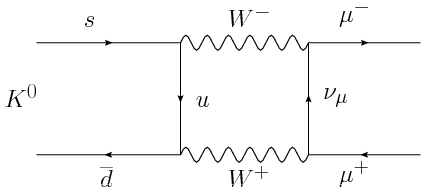
\includegraphics[width=0.5\textwidth]{Glashow-Illiopoulos-Maiani_mechanism_fig1.png}
	\caption{Box diagram describing $K_L^0\rightarrow\mu^-\mu^+$, through an intermediate $u$ quark. \Joao{A imagem tem pouca qualidade. Consegues fazer isto no latex com a package feynmp. No tutorial que te enviei tem lá o código}}
	\label{fig:Kaon}
\end{figure}

\Joaoout{We avoided discussing leptons since in the SM their mass eigenstates can be easily shown to have no real consequence besides a change of basis.} 
%
\Joaorep{You}{We} might also note a very interesting feature of the Standard Model, by consequence of the $\mathrm{SU(2)_L \times U(1)_Y }$ symmetry\Joaoadd{. T}here are no interactions of the right handed unitary matrices and \Joaorep{there for}{thus} no mixing, coupling, or charged currents of right handed quarks, making them theoretically invisible to measurements. \Joao{Já notei que às vezes usas ``you''. Não te dirigas para o arguente ou para que está a ler. Tenta usas sempre expressões com ``We''}
%
\begin{figure}[H]
	\centering
	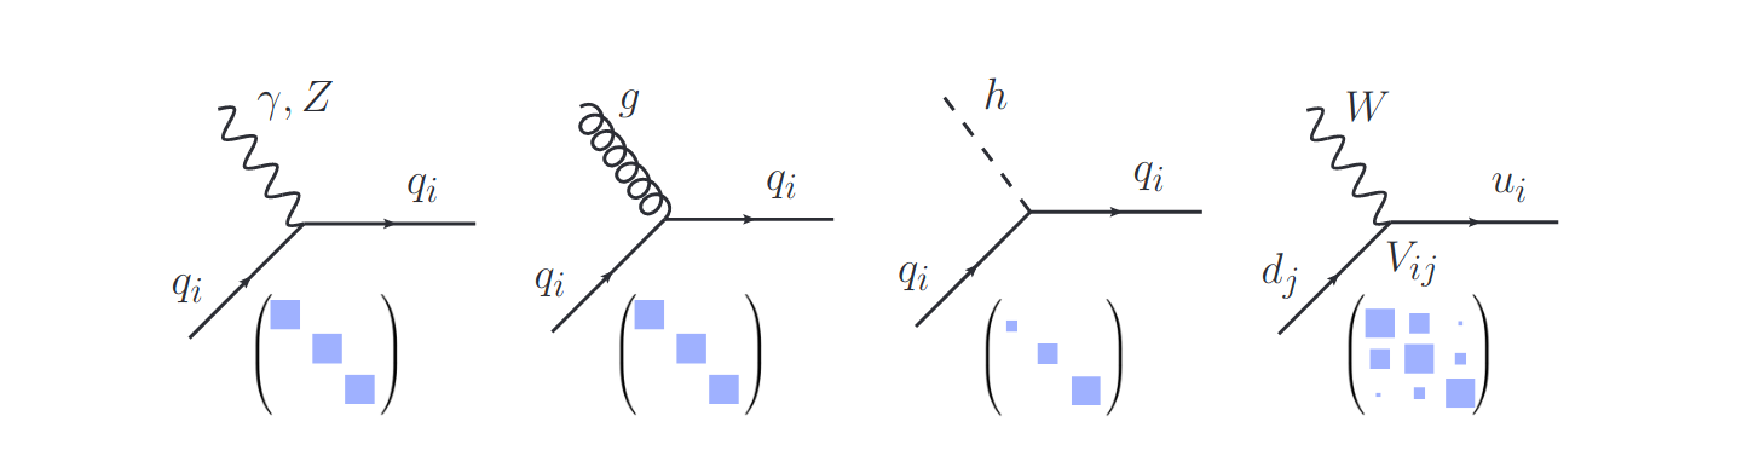
\includegraphics[width=0.9\textwidth]{TestYukawaCouplings.pdf}
	\caption{\Joaoout{The} Feynman diagrams for flavour conserving couplings of quarks to photon, $Z$ boson, gluon and the Higgs (the first three diagrams), and the flavour changing coupling to the $W$ (the last diagram). The $3\times3$ matrices are visual representations of couplings in the generation space, with couplings to $\gamma$, $Z$, $g$ \Joaoadd{being} flavour universal, \Joaorep{the}{while} couplings to the Higgs flavour \Joaoadd{are} diagonal but not universal\Joaorep{, and the couplings to}{. The couplings involving} $W$ \Joaoadd{are} flavour changing and hierarchical.}
	\label{fig:QuarkCKM}
\end{figure}
%

% Possible power gap
%
% Here we introduce the CKM matrix, a $3 \times 3$ unitary matrix. It is a paramatrization of the three mixing angles and CP-violating KM phase. There are many possible conventions to represent the CKM matrix. 

The CKM matrix elements are fundamental parameters of the particle physics, so their precise determination is important, and reproducing the quark mixing parameters is fundamental for BSM searches that include changes to how the quarks interact with possible new Higgs bosons. 
 

\subsection{Charged Flavour Currents vs. Neutral Flavour Currents}

In the SM there is a very important distinction between flavour changing neutral and charged currents. \Joaoout{Flavour Changing Neutral Currents} FCNCs are processes in which the quark flavour changes, while the quark charge stays the same. 
%
The Flavour Changing Charged Currents (FCCCs) change both the flavour and the charge of the quark. 
%
Extracting some representative probabilities from \cite{Tanabashi:2018oca} reveals that the two types of processes are strikingly different.  
%
The charged currents lead to the dominant weak decays, while the FCNC\Joaoadd{s} induce\Joaoout{d} decays \Joaoadd{that} are extremely suppressed. Rounding the experimental results, and not showing the errors, a few representative decays are, 
%
\setlength{\tabcolsep}{2pt} % Default value: 6pt
\renewcommand{\arraystretch}{1} % Default value: 1
%
\begin{table}[!htb]
    %\caption{Global caption}
    \begin{minipage}{.5\linewidth}
      \caption{FCCCs examples}
\centering
\begin{tabular}{lcl}
$s \rightarrow u \mu^- \nu_\mu $ & : & Br $\left( K^+ \rightarrow \mu^- \nu\right) = 64 \%$                 \\
$b \rightarrow c l^- \nu_l $       & : & Br $\left( B^- \rightarrow D^0 l \overline{\nu}_l \right) = 2.3 \% $ \\
$c \rightarrow u \mu^- \nu_\mu $   & : & Br $\left( D^\pm \rightarrow K^0 \mu^\pm \nu \right) = 9 \%$        
\end{tabular}
    \end{minipage}%
    \begin{minipage}{.5\linewidth}
      \centering
        \caption{FCNCs examples}
\begin{tabular}{lcl}
$s \rightarrow d \mu^+ \mu^- $ & : & Br $\left( K_L \rightarrow\mu^+ \mu^- \right) =  7\times10^{-9}$        \\
$ b \rightarrow d \mu^+ \mu^-$ & : & Br $\left( B^- \rightarrow  K^{\** -} l^+ l^- \right) =  5\times10^{-7}$ \\
$ c \rightarrow u l^+ l^-$     & : & Br $\left( D^0 \rightarrow \pi l^+ l^- \right) =  1.8\times10^{-4}$      
\end{tabular}
    \end{minipage} 
\end{table}

\setlength{\tabcolsep}{6pt} % Default value: 6pt
\renewcommand{\arraystretch}{1} % Default value: 1

The reason for such a striking difference is that in the SM the charged currents occur at tree level, while FCNCs are forbidden at tree level and only arise starting at one loop order\Joaoadd{. N}ote the lack of neutral couplings between the up and down families in Eq \ref{LagFermFCCCs}. The relative complexity of these processes can be easily seen in Fig \ref{fig:Flavour_D_1},
%
\begin{figure}[H]
	\centering
	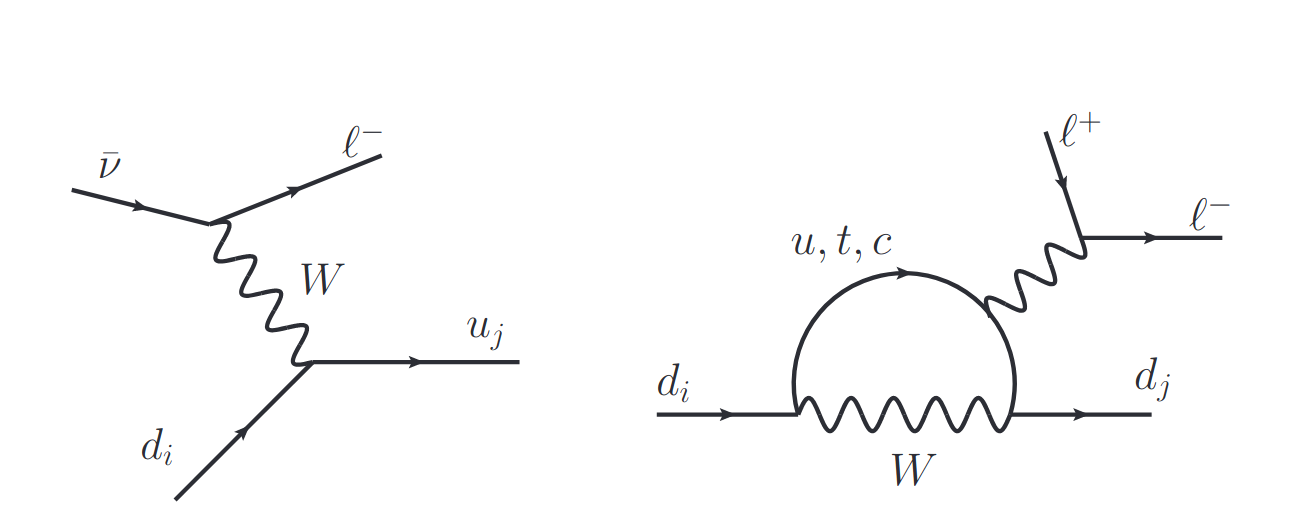
\includegraphics[width=0.75\textwidth]{Stolen.png}
	\caption{Representative tree level charged current diagram (left) and a loop induced FCNC diagram (right).}
	\label{fig:Flavour_D_1}
\end{figure}
%
%Making FCNCs virtual process.
%
Furthermore, the FCNCs come suppressed by the difference of the masses of the quarks running in the loop, $m^2_j-m^2_i$. This so called Glashow-Iliopoulos-Maiani (GIM) mechanism \cite{glashow1970weak}. Given the \Joaoadd{differences} between the masses of the up and down sectors, \Joaorep{it}{this} has a significant impact. 
%
A interesting result of this mechanism would be that that there is no flavour violation, if all the quark masses are the same.

\subsubsection{Flavour as a Probe into New Physics}

Now that we have introduced \Joaorep{without great detail}{a bit of} flavour physics we can briefly touch on why collider experiments have been sold \Joaoout{a} as a pathway to discovering new physics i.e. how deviation in rare decays could pin point exactly what is missing in the \Joaorep{Standard Model}{SM}. 

Thanks to these large experiments we have many new observables in flavour physics, e.g. \Joaoout{the} branching ratios, asymmetries, distributions \Joao{Que asimetrias? Que distribuições? Diz em específico}. For each of these examples there is also a plethora of different parent particles for each change of flavour, as well as many instances of final states. 
%
The abundance of observables is clearly illustrated by opening the handy Particle Data Group (PDG) book \Joao{Alterei citação para aparecer todos os nomes}\cite{Tanabashi:2018oca}.\Joaoout{where even the condensed version, the PDG booklet, clocks out at more than 170 pages of mostly tabled information about these observables.}

%To shorten the discussion we will focus on the processes that are at present showing deviations from the SM expectations. 

The recipe then, seems simple, identify processes that are rare in the SM and then search for deviations from the SM predictions. However\Joaoadd{,} thus far\Joaoadd{,} all but two processes are within $2\sigma$ experimental and theoretical bounds given by the SM. 
%
These are the $b \rightarrow s \mu \mu$ and $b \rightarrow c \tau \nu$ channels. They are, so far, showing over $ 4 \sigma$ deviations from \Joaoout{the} their expected value. {\color{blue} (citation needed \Joao{Damn right you are!})}.
%
Without going into too much depth onto the NP searches, we can examine the scale at which these processes are "integrated away". This is the energy scale at which a NP vector-axial operator would allow these processes to exist only at high energies. These energies are naturally high given the terms in \eqref{eq:NP}. 
% Avoiding going in depth into these processes, what this might point us too, by these processes as suppressed the vector-axial processes. For them to be integrated away we get very different, but high, energy scales. There would have to exist terms a kin to, 
%If examined through V-A operators the NP scale of these 2 processes are both very different and very heavy, these would be something a kin to, 
%
\bigbreak
%
\noindent\begin{minipage}{.3\textwidth}
	\begin{figure}[H]
		\label{fig:contactNP}
		\centering
		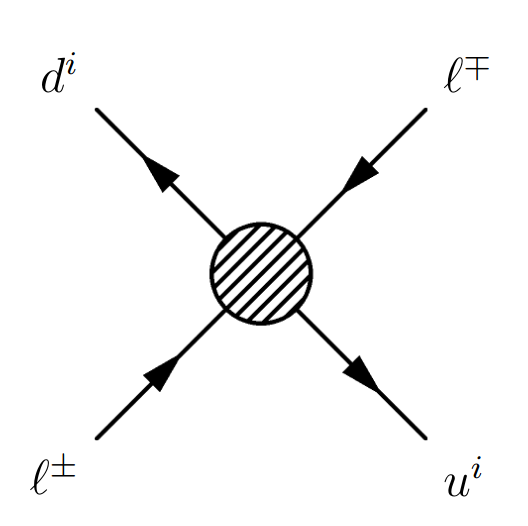
\includegraphics[width=0.65\textwidth]{My_First_Diagram.png}
		\caption{"Contact" interactions with loop interactions containing NP}
	\end{figure}
\end{minipage}
\begin{minipage}{.6\textwidth}
\begin{equation}
\label{eq:NP}
\mathcal{L}_{NP} \supset \frac{1}{\Lambda_{NP}} (\bar{Q}_i \gamma^\mu \sigma^A Q_j ) (\bar{L}_k \gamma_\mu \sigma^A L_l) 
\end{equation}
\end{minipage}
%
\bigbreak
%
\Joao{O que é o $\sigma^A$? Não existe nada a contrair os índices de flavour, é mesmo assim? O $A$ também é um índice livre} To explain $b \rightarrow s \mu \mu$ transitions you would need a $\Lambda_{NP} \approx 3 \ \text{TeV}$ while for $b \rightarrow c \tau \nu$ you would need a $\Lambda_{NP} \approx 30\ \text{TeV}$ \Joao{Podes explicar? Eu não sei.}. This is a strong indicator that some components are missing in our formulation like a new mediator for gauge interactions. \Joaorep{And the}{The} advantage of this scale is \Joaoout{it} almost certainly in most BSM scenarios, avoiding most experimental constraints.

As for the FCNC diagram \Joaoout{for}, the $b \rightarrow s \mu \mu$ channel can be seen in Fig \ref{fig:Flavour_D_2_Muon}, 
%
\begin{figure}[H]
	\centering
	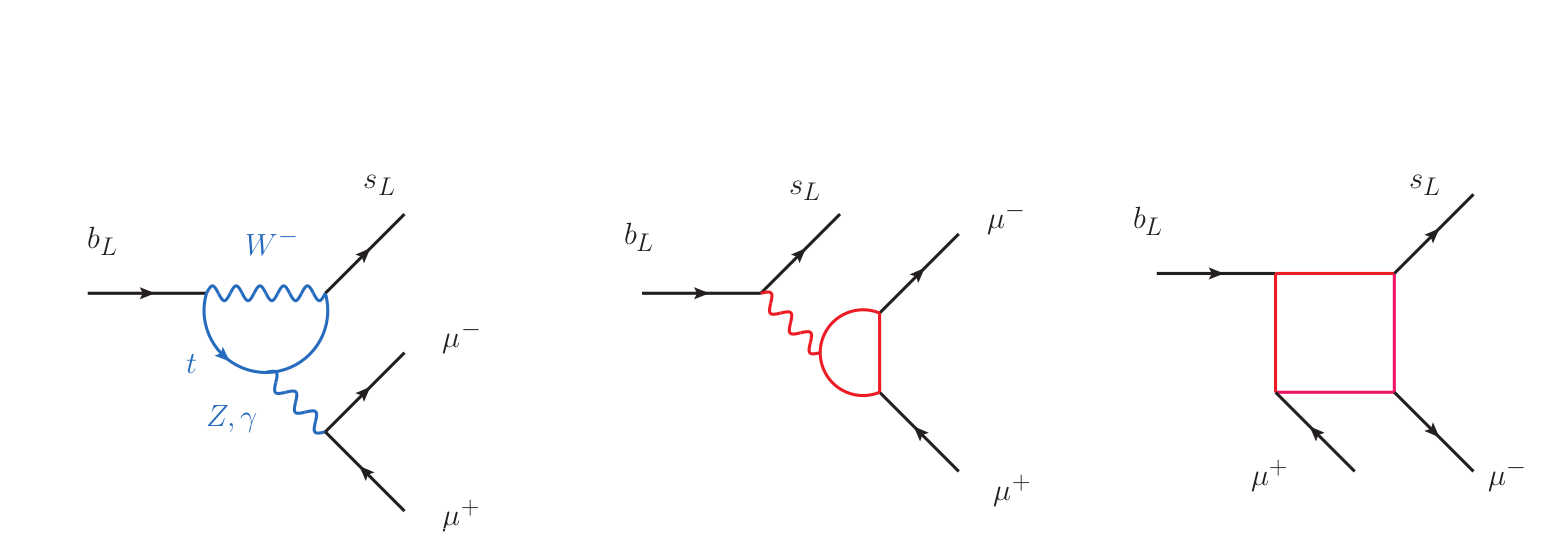
\includegraphics[width=0.75\textwidth]{Stolen_2.png}
	\caption{A representative SM diagram for $b \rightarrow s \mu \mu$ transition (left), and representative possible loop level NP
contributions (middle and right).}
	\label{fig:Flavour_D_2_Muon}
\end{figure}
%
The $b \rightarrow c \tau \nu$ flavour anomaly is similarly very clean theoretically \cite{Fajfer_2012}. However, the NP effect in these diagrams is large {\color{blue} (citation needed)} and often this means that the scale of NP needs to be lower than in the previous case. Consequently the NP interpretations here are often in conflict with experimental constraints {\color{blue} (citation needed)}.
%
This means the most obvious candidates are ruled out. Theoretical bias would have been that the new charged currents are either due to a charged Higgs, $H^+$ , or a new vector boson, $W^\prime$, see Fig. \ref{fig:Flavour_D_3_Tau} {\color{blue} (citation needed)}.
%
\begin{figure}[H]	
	\centering
	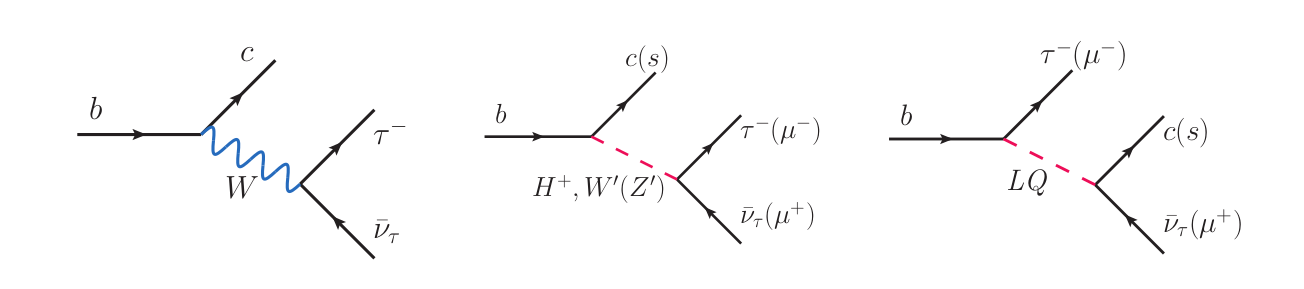
\includegraphics[width=0.75\textwidth]{Stolen_3.png}
	\caption{The SM diagrams for $b \rightarrow c \tau \nu$ transition (left), and the possible tree level NP contributions to $b \rightarrow c \tau \nu$ transition (middle and right). \Joao{Não disses o que é o LQ. É um leptoquark?}}
	\label{fig:Flavour_D_3_Tau}
\end{figure}
%
Another prediction of the SM is that the rates for the  $b \rightarrow s e^+ e^-$ and  $b \rightarrow s \mu^- \mu^+$ transitions should be equal to each other.
%
The SM prediction of Lepton Flavour Universality (LFU) is deeply engrained in the structure of the theory, since it is a consequence of the fact that the electroweak gauge group is the same for all three generations. 
%
The prediction of LFU can be tested experimentally, also trough flavour physics, by theoretically clean observables such as the ratios \Joaoout{of these flavour observables,} 
%
\begin{equation}
R_{K^{\**}} = \frac{\text{Br}( B \rightarrow K^{\**} \mu^- \mu^+ )}{\text{Br} (  B \rightarrow K^{\**} e^- e^+  )}.
\end{equation}
% 
Another strong indicator of new physics is the fact the experimental value for this ratio is $R_{K^{\**}} \approx 0.7$, violating LFU by $2.2 - 2.6 \sigma$ {\color{blue} (citation needed)}.

\subsubsection{The Future of Flavour Indirect Searches}

The NP searches with rare decays \Joaorep{, as well boost with the upcoming}{will benefit from the upcoming upgrades at} Belle II and \Joaoadd{the} LHC \Joaoout{upgrades}. Belle II expects to collect 50 times the Belle dataset. First collisions were seen in May 2018, and the first B physics run is expected in March 2019. While for the LHC, after upgrade II aims for roughly 100 times the present data set with an upgraded detector. {\color{blue} (citation needed)}.
%
%A rule of thumb on the improved NP reach gives, for instance for Belle II, that the reach in $\Lambda_NP$ will be improved by $\sqrt[4]{50} \approx 2.7$. Similar if not larger increase applies to LHCb Upgrade II sensitivity improvements. This is a similar jump in energy reach as going from 13 TeV LHC to a 35 TeV LHC!
%
Undoubtedly this improvement in sensibility will translate to a finer value for all measurable parameters at these experiments. We expect these anomalies then to go over the required $5 \sigma$ in future experiments (Assuming of course, they are not statistical deviations). {\color{blue} (citation needed)}.



\newpage 

% 
% Introduction of the BLSM.  
% 
% 

%\section{B-L-SM Model}
\chapter{B-L-SM Model} 
\label{Chap:B-L-SM_Model}

% Got this from the abstract in my BLSM paper 

%Here we start the our first look at BSM scenarios. 
%
In this chapter we introduce the minimal $\U{B-L}$ gauge extension of the SM named, the B-L-SM (Baryon-Lepton-SM) Model \cite{Mohapatra:1980qe,Basso:2010hk,Basso:2011na}. 
%
In this model, we are capable of explaining the generation of neutrinos masses generation via a simple see-saw mechanism. Additionally, by virtue of two new physical states, specifically a new Higgs like boson $\mathrm{H}^\prime$ and a $\mathrm{Z}^\prime$ gauge boson we can also address other phenomenology, such as deviations in EW measurements, namely the $(g-2)_\mu$ anomaly \cite{Tanabashi:2018oca}. 

The additional bosons aquire mass primarily trough the spontaneous breaking of the $\U{B-L}$ symmetry that gives it's name to the model.
%
This unitary group originates from the promotion of an accidental symmetry present in the SM, the Baryon number (B) minus the Lepton number (L) to a fundamental Abelian symmetry group. 
%
This origin for the mass of the referenced bosons means the model is already very heavily constrained due to long-standing direct searches at the LHC. 

Through this model we can address the metastability of the EW vacuum in the SM trough the new scalar. Allowing for Higgs stabilization up to the Plank scale with a new Higgs starting from a few hundred GeVs \cite{Degrassi:2012ry,Alekhin:2012py,Buttazzo:2013uya}. 

The B-L-SM framework is particular interesting in the context of the study of Grand Unified Theories (GUT) as it easily embedded into higher order symmetry groups like the $\mathrm{SO(10)}$ \cite{Chanowitz:1977ye,Fritzsch:1974nn,Georgi:1978fu,Georgi:1979dq,Georgi:1979ga} or $\mathrm{E}_6$ \cite{Achiman:1978vg,Gursey:1975ki,Gursey:1981kf} Lie groups.   
The presence of a new complex singlet field, $\chi$, with a Higgs doublet typically results in enhanced strength of the EW phase transition potentially converting it into a strong first-order one. This would be could be detectable in the form of a gravitational wave background \cite{Barger:2008jx}. 
%
Such a analysis is of utmost importance given that it could provide a way to detect NP or exclude models without the need for a larger particle collider. % but instead a sensitive probe also capable of studying gravitational events. 

However, a family-universal symmetry such as $\mathrm{U(1)_{B-L}}$, being introduced without changing the SM fermion content would lead to chiral anomalies. This translates to a non conservative charged current on some channels involving the $\mathrm{U(1)_{B-L}}$. These are not completely undesired by themselves, as they would allow for the presence of extra sources of $\mathcal{CP}$ violation, but this inclusion at tree-level without a suppression mechanism would lead to far too much $\mathcal{CP}$ violation. 

The model also benefits from the presence of three generations of right-handed heavy Majorana neutrinos that through the new field additions are possible in a framework free of anomalies while also allowing for a minimal see-saw mechanism that generates light neutrino masses unlike the SM.  \cite{Yanagida:1979as,GellMann:1980vs,Mohapatra:1979ia}.´
%
The mass scale of such neutrinos is established once the $\U{B-L}$ symmetry is broken. 
%
These neutrinos are of cosmological significance given their presence could imply the existence of a sterile state that can play the role of Dark Matter \cite{Kaneta:2016vkq}.
%
The relatively small alteration of a, $\mathbb{Z}_2$, symmetry in the neutrino sector can make these fully sterile, as seen in \cite{Okada:2010wd,Okada:2018ktp}. {\color{red} Check if the Z2 affects the Zprime, if so we must comment that it doens't allow kinetic mixing! and would alter the $a_\mu$. Acho que não. Não deve haver alterações dos couplings com o muão, portanto a um loop não acontece nada. A dois loops, também não deve haver, pois os neutrinos não tem carga e não acoplam ao fotão, dos diagramas que aparecem na Fig. 4.7 Preciso mesmo de falar com o morais para ter a certeza.}
%
These neutrinos can, in such case, be used to help explain the baryon asymmetry via the leptogenesis mechanism, this scenario is discussed in depth in the following Refs.~\cite{Fukugita:1986hr,Pilaftsis:1997jf,Pilaftsis:2003gt}. 

With this in mind, we structure this chapter in the fol-
lowing way. First, we present the fundamental theoretical background on the model with a strong focus on the basic details of the scalar and the gauge boson mass spectra and mixing. Followed by a modern precise study of the phenomenological status of the B-L-SM model trough a layered algorithm that will be discussed preceding the results. With this algorithm we provide a numerical analysis that tests the relevant phenomenological constraints in direct and EW observables. FFollowed by this study, we table off a few representative benchmark points. 

% { \color{blue} perhaps I should include this on the start of the chapter  }

\section{Formulating the model}

Essentially, the minimal B-L-SM is a BSM framework containing only three new ingredients, a new gauge interaction given the new symmetry group, three generations of right handed neutrinos, and a complex scalar field $\chi$. 

The first of these is well motivated by the aformentioned GUT scenarios, While a new sector of additional three $\mathrm{U(1)_{B-L}}$ charged Majorana neutrinos is essential for anomaly cancellation.
%The first of these, is motivated by the aforementioned GUT scenarios, as seen in the Refs, \cite{Chanowitz:1977ye,Fritzsch:1974nn,Georgi:1978fu,Georgi:1979dq,Georgi:1979ga,Achiman:1978vg,Gursey:1975ki,Gursey:1981kf}, here you can see that the B-L-SM can be introduced in a large number of groups, like $E_6$ and $\mathrm{SO}(10)$. 
%
%Secondly, as mentioned, a new sector of additional three $U(1)_{B-L}$ charged Majorana neutrinos is essential for anomaly cancellation and addresses many concerns of the SM. 

Finally, the SM-like Higgs doublet, $H$, does not carry neither baryon nor lepton number, this way it does not participate in the breaking of $\mathrm{U(1)_{B-L}}$. It is then necessary to introduce a new scalar singlet field, $\chi$, solely charged under $\mathrm{U(1)_{B-L}}$, to perform the breaking of the $\mathrm{B-L}$ symmetry.

The particle content and related charges of the minimal $U(1)_{B-L}$ extension of the SM are shown in Tab \ref{tab:BLSM_Charges}. Note these are similar to the SM as to be expected. 
%
\begin{table}[H]
\centering
\begin{tabular}{|c|c|c|c|c|c|c|c|c|}
\hline
  & $q_L$  & $u_R$ & $d_R$ & $l_L$  & $e_R$ & $\nu_R$  &  $H$  & $\chi$  \\ \hline
 $\mathrm{SU(3)_C}$& $\mathbf{3}$ & $\mathbf{3}$  & $\mathbf{3}$  & $\mathbf{1}$  & $\mathbf{1}$   & $\mathbf{1}$   & $\mathbf{1}$    & $\mathbf{1}$    \\
 $\mathrm{SU(2)_L}$& $\mathbf{2}$  & $\mathbf{1}$ & $\mathbf{1}$ & $\mathbf{2}$ & $\mathbf{1}$ & $\mathbf{1}$ & $\mathbf{2}$  & $\mathbf{1}$ \\
$\mathrm{U(1)_Y}$ & ${1}/{6}$ & ${2}/{3}$  & -${1}/{3}$  & -${1}/{2}$ & -1 & 0 & ${1}/{2}$ & 0 \\
$\mathrm{U(1)_{B-L}}$ & ${1}/{3}$ & ${1}/{3}$ & ${1}/{3}$  & -1  & -1 &-1  & 0 & 2  \\ \hline 
\end{tabular}
\caption{Quantum fields and their respective quantum numbers in the minimal B-L-SM extension. The last two lines represent the weak and $B-L$ hypercharges}
\label{tab:BLSM_Charges}
\end{table} 

\subsubsection{Scalar sector}

With the information from Tab \ref{tab:BLSM_Charges}, we can begin examining the new Lagrangian terms. Starting by the scalar potential, which now depends on two fields, 
%
\begin{equation}
\label{eq:potential}
V(H,\chi) = \mu_1^2 H^\dagger H + \mu_2^2 \chi^\ast \chi + \lambda_1 (H^\dagger H)^2 + \lambda_2 \left(\chi^\ast \chi\right)^2 + \lambda_3  \chi^\ast \chi H^\dagger H , 
\end{equation}
%
where,  $\lambda_i$, the scalar couplings and $\mu_{1,2}^2$ the quadratic terms for $H$ and $\chi$ respectively. This potential must lead to a stable vacuum state, which means that the scalar potential must be bounded from below (BFB), as to ensure a global minima.  Studying the potential on Eq.\,(\ref{eq:potential}) we deduce the conditions,
\begin{equation}
4 \lambda_1 \lambda_2  -  \lambda_3^2 > 0 \quad , \quad \lambda_1 , \lambda_2>0 
\label{eq:BFB}
\end{equation}
%
Where the full components of the scalar fields $H$ and $\chi$ are given by,
\begin{equation}
H = \frac{1}{\sqrt{2}} 
\begin{pmatrix}
-i \( \omega_1 - i \omega_2 \) \\
v + (h + i z)
\end{pmatrix} \quad \chi = \frac{1}{\sqrt{2}} \( x + \(h^\prime + i z^\prime\) \)
\end{equation}
%
where we note that the parameters $v$ and $x$ are VEV’s associated with the $H$ field and the $\chi$ field, respectively.
In these equations we can see that $h$ and $h^\prime$ represent the radial quantum fluctuations around the minimum of the potential. These will constitute the physical degrees of freedom associated with $H$ and $H^\prime$. There are also four Goldstone directions denoted as $\omega_1$, $\omega_2$, $z$ and $z^\prime$ which are absorbed into longitudinal modes of the $W^\pm$, $Z$ and $Z^\prime$ gauge bosons once SSB takes place. After SSB the associated VEVs take the form, 
%
\begin{equation}
 \langle H \rangle = \frac{1}{\sqrt{2}} 
\begin{pmatrix}
0 \\
v 
\end{pmatrix}	
\qquad
 \langle  \chi \rangle  = \frac{x}{\sqrt{2}}
\label{eq:vacuum}
\end{equation}
% 
%here, recall $v$ and $x$ are the associated VEVs to each field. 
From here we can solve the tadpole equations in relation to each of the VEVs as to ensure non-zero VEV. We arrive at,
%
\begin{equation}
	v^2 = \tfrac{-\lambda_2 \mu_1^2 + \tfrac{\lambda_3}{2}\mu_2^2}{\lambda_1 \lambda_2 - \tfrac{1}{4}\lambda_3^2} > 0
	\qquad
	\text{and}
	\qquad
	x^2 = \tfrac{-\lambda_1 \mu_2^2 + \tfrac{\lambda_3}{2}\mu_1^2}{\lambda_1 \lambda_2 - \tfrac{1}{4}\lambda_3^2} > 0 
	\label{eq:extremum}
\end{equation}
%
which, when simplified with the BFB conditions yield a simpler set of equations,
%
\begin{equation}
\lambda_2 \mu_1^2 < \tfrac{\lambda_3}{2} \mu_2^2 
\qquad
\text{and}
\qquad
\lambda_1 \mu_2^2 < \tfrac{\lambda_3}{2} \mu_1^2
\label{eq:sols}
\end{equation}
%
Note that although $\lambda_1$ and $\lambda_2$ must be positive to ensure the correct conical shape of the potential, no such conditions exist for the sign of $\lambda_3$ , $\mu_1$, and $\mu_2$. However observing Eq\,(\ref{eq:sols}) we can infer that only some combinations of signs are impossible, 
%
\begin{table}[H]
	\begin{center}
		\begin{tabular}{ccccc}
			& $\mu_2^2 > 0$ & $\mu_2^2 > 0$ & $\mu_2^2 < 0$ & $\mu_2^2 < 0$  	\\
			& $\mu_1^2 > 0$ & $\mu_1^2 < 0$ & $\mu_1^2 > 0$ & $\mu_1^2 < 0$  	\\        
			\hline  
			$\lambda_3 < 0 $     			    							& \xmark		& \checkmark	&	\checkmark & \checkmark	\\
			$\lambda_3 > 0$     			    							& \xmark		& \xmark	&	\xmark &  \checkmark \\
			\hline
		\end{tabular} 
		\caption{Possible signs of the potential parameters in Eq\,(\ref{eq:potential}). 
The \checkmark\,symbol indicates the existence of solutions for tadpole conditions Eq.\,(\eqref{eq:sols}), while the \xmark\,indicates unstable configurations.}
		\label{tab:signs}  
	\end{center}
\end{table} 
%
For our numerical analysis we decided to leave the sign of $\lambda_3$ positive, choosing a configuration where both $\mu$ parameters are negative. 
%
This does not directly translate to any real physical consequence.  
%
With these conditions now established we proceed to investigate the physical states of the B-L-SM scalar sector. 
%
At the vacuum, we evaluate the Hessian matrix as,
%
\begin{equation}
\mathbf{M}^2 =
\begin{pmatrix}
4 \lambda_2 x^2 & \lambda_3 v x \\ 
\lambda_3 v x   & 4 \lambda_1 v^2 
\end{pmatrix}\,,
\label{eq:hess}
\end{equation}
% 
Moving this matrix to its physical mass eigen-base, we obtain the following eigenvalues,
%
\begin{equation}
m_{h_{1,2}}^2 = \lambda_1 v^2 + \lambda_2 x^2 \mp \sqrt{(\lambda_1 v^2 - \lambda_2 x^2)^2 + (\lambda_3 x v)^2}.
\label{eq:eigvals}
\end{equation}
The physical basis vectors $h_1$ and $h_2$ can then be related to the original fields of gauge eigen-basis $h$ and $h^\prime$ trough a simple rotation matrix:
%
\begin{equation}
	\begin{pmatrix}
	h_1 \\
	h_2 
	\end{pmatrix}
	=
	\mathbf{O}
	\begin{pmatrix}
	h \\
	h^\prime 
	\end{pmatrix},
	\label{eq:trans}
\end{equation}
%
where $\mathbf{O}$ can be parameterized by a single mixing angle $\alpha_h$,
%
\begin{equation}
	\mathbf{O} = 
	\begin{pmatrix}
	\cos \alpha_h & -\sin \alpha_h \\
	\sin \alpha_h & \cos \alpha_h 
	\end{pmatrix}\,.
	\label{eq:rotmat}
\end{equation}
%
The precise mixing angle is represented simply by, 
\begin{equation}
\tan 2 \alpha_h   = \frac{ \left| \lambda_3 \right|  v x }{  \lambda_2 x^2 -\lambda_1 v^2 } 
\end{equation} 
%
It is particularly interesting to analyse the scenario where the scalar fields approximately decouple, that is, in the limit, $v/x\ll 1$. In these circumstances, the scalar masses and the mixing angle become rather simple,
\begin{equation}
\sin \alpha_h \approx \dfrac{1}{2}\dfrac{\lambda_3}{\lambda_2} \dfrac{v}{x} \qquad
m_{h_1}^2 \approx 2 \lambda_1 v^2 \qquad m_{h_2}^2 \approx 2 \lambda_2 x^2
\label{eq:simplify}
\end{equation}
%
We will see in the context of our numerical results that for a phenomenologically consistent mass scale these equations serve as a valid approximation for most of the  points. 

\subsubsection{Gauge Sector}

Moving onto the gauge boson and Higgs kinetic terms in the B-L-SM, consider the following portion of the Lagrangian,
\begin{equation}
\mathcal{L}_{\mathrm{U(1)'s}} =  \left| D_\mu H \right|^2 + \left| D_\mu \chi \right|^2 -\dfrac{1}{4} F_{\mu \nu} F^{\mu \nu} -\dfrac{1}{4} F^\prime_{\mu \nu} F^{\prime \mu \nu} -\dfrac{1}{2} \kappa F_{\mu \nu} F^{\prime \mu \nu}
\label{eq:Lu1}
\end{equation}
where $F^{\mu \nu}$ and $F^{\prime \mu \nu}$ are the standard field strength tensors, respectively for the $\U{Y}$ and  $\U{B-L}$ Abelian groups, 
\begin{equation}
	F_{\mu \nu} = \partial_\mu A_\nu - \partial_\nu A_\mu 
	\qquad
	\text{and}
	\qquad
	 F^\prime_{\mu \nu} = \partial_\mu A^\prime_\nu - \partial_\nu A^\prime_\mu\,.
	 \label{eq:Fmn}
\end{equation}
written in terms of the gauge fields $A_\mu$ and $A_\mu^\prime$, respectively. Given that this is a model with two Unitary groups, without a parity symmetry ($\mathbb{Z}_2$) to prevent it, we must consider the possible mixing in between them. In this work we parameterized this mixing trough a parameter $\kappa$.

The Abelian part of the covariant derivative in Eq.\,( \ref{eq:Lu1}) is given by,
\begin{equation}
	D_\mu \supset i g_1 Y A_\mu + i g_1^\prime Y_{\rm B-L} A_\mu^\prime\,,
\end{equation} 
% 
with $g_1$ and $g_1^\prime$ the $\U{Y}$ and $\U{B-L}$ the gauge couplings with the $Y$ and $B-L$ charges are specified in Tab.~\ref{tab:charges}. It is convenient to rewrite the gauge kinetic terms in the canonical form, i.e.
%
\begin{equation}
	F_{\mu \nu} F^{\mu \nu} + F^\prime_{\mu \nu} F^{\prime \mu \nu} + 2 \kappa F_{\mu \nu} F^{\prime \mu \nu} \to B_{\mu \nu} B^{\mu \nu} + B^\prime_{\mu \nu} B^{\prime \mu \nu}\,.
	\label{eq:AtoB}
\end{equation}
%
A generic orthogonal transformation in the field space does not eliminate the kinetic mixing term. So, in order to satisfy Eq.~\eqref{eq:AtoB} an extra non-orthogonal transformation should be imposed such that Eq.~\eqref{eq:AtoB} is realized. Taking $\kappa = \sin \alpha$, a suitable redefinition of fields $\{A_\mu,A_\mu^\prime\}$ into $\{B_\mu, B_\mu^\prime\}$ that eliminates $\kappa$-term according to Eq.~\eqref{eq:Lu1} can be cast as
\begin{equation}
	\begin{pmatrix}
	A_\mu \\
	A^\prime_\mu 
	\end{pmatrix}
	=
	\begin{pmatrix}
	1 & -\tan \alpha \\
	0 & \sec \alpha 
	\end{pmatrix}
	\begin{pmatrix}
	B_\mu \\
	B^\prime_\mu 
	\end{pmatrix}\,,
	\label{eq:trans-kappa}
\end{equation}
Note there is a limit without kinetic mixing where $\alpha = 0$. Note that this transformation is generic and valid for any basis in the field space. The transformation (\ref{eq:trans-kappa}) results in a modification of the covariant derivative that acquires two additional terms encoding the details of the kinetic mixing, i.e.

\begin{equation}
D_\mu \supset \partial_\mu + i \(g_Y \; Y + g_BY \; Y_{B-L}\) B_\mu + i \(g_{B-L} \; Y_{B-L} + g_{YB} \; Y\) B_\mu^\prime\,,
\label{eq:newCov}
\end{equation}	
where the gauge couplings take the form
\begin{equation}
	\begin{cases}
	g_Y = g_1 \\
	g_{B-L} = g_1^\prime \sec \alpha \\
	g_{YB} = -g_1 \tan \alpha \\
	g_{BY} = 0
	\end{cases} \,,
	\label{eq:new-g-simp}
\end{equation}
which is the standard convention in the literature. Note that this definition is merely to simplify the equations and has no physical impact. We will later see that this kinetic mixing is a desired feature and why stabilizing it with a $\mathbb{Z_2}$ symmetry would be detrimental in terms of depth. The resulting mixing between the neutral gauge fields including $Z^\prime$ can be represented as follows
%
\begin{equation}
\begin{aligned}
\begin{pmatrix}
\gamma_\mu \\
Z_\mu \\
Z^\prime_\mu
\end{pmatrix}
=
\begin{pmatrix}
\cos \theta_W & \sin \theta_W & 0\\
-\sin \theta_W \cos \theta_W^\prime & \cos \theta_W \cos \theta_W^\prime & \sin \theta_W^\prime \\
\sin \theta_W \sin \theta_W^\prime & -\cos \theta_W^\prime \sin \theta_W^\prime & \cos \theta_W^\prime
\end{pmatrix}
\begin{pmatrix}
B_\mu \\
A^3_\mu \\
B^\prime_\mu
\end{pmatrix}
\end{aligned}
\label{eq:g-Z-Zp}
\end{equation}	
%
where $\theta_W$ is the weak mixing angle and $\theta^\prime_W$ is defined as
\begin{equation}
\sin(2 \theta^\prime_W) = \frac{2 g_{YB} \sqrt{g^2 + g_{Y}^2}}{\sqrt{(g_{YB}^2 + 16 (\frac{x}{v})^2 g_{B-L}^2 - g^2 - g_{Y}^2)^2 + 4 g_{YB}^2 (g^2 + g_{Y}^2)} }\,,
\label{eq:theta-p-full}
\end{equation}
%
in terms of $g$ and $g_{Y}$ being the $\mathrm{SU(2)_{L}}$ and $\mathrm{U_{Y}}$ gauge couplings, respectively. In the physically relevant limit, $v/x \ll 1$, the above expression greatly simplifies leading to
%
\begin{equation}
	\sin \theta_W^\prime \approx \dfrac{1}{16
	} \dfrac{g_{YB}}{g_{B-L}}\( \dfrac{v}{x} \)^2 \sqrt{g^2 + g_{Y}^2} \,,
	\label{eq:theta-p}
\end{equation}
%
up to $(v/x)^3$ corrections. In the limit of no kinetic mixing, i.e. $g_{YB} \to 0$, there is no mixture of $Z^\prime$ and SM gauge bosons. 

Note, that the kinetic mixing parameter $\theta_W^\prime$ has rather stringent constraints from $Z$ pole experiments both at the Large Electron-Positron Collider (LEP) and the Stanford Linear Collider (SLC), restricting its value to be smaller than $10^{-3}$ approximately \cite{Bandyopadhyay_2018}, which we set as an upper bound in our numerical analysis. Expanding the kinetic terms $\left| D_\mu H \right|^2 + \left| D_\mu \chi \right|^2$ around the vacuum one can extract the following mass matrix for the vector bosons
\begin{equation}
	m_V^2 =
	\dfrac{v^2}{4}
	\begin{pmatrix}
	g^2 \;\;&\;\; 0 \;\;&\;\; 0 \;\;&\;\; 0 \;\;&\;\; 0 \\
	0 \;\;&\;\; g^2 \;\;&\;\; 0 \;\;&\;\; 0 \;\;&\;\; 0 \\
	0 \;\;&\;\; 0 \;\;&\;\; g^2 \;\;&\;\; -g g_{Y} \;\;&\;\; -g g_{YB} \\
	0 \;\;&\;\; 0 \;\;&\;\; -g g_{Y} \;\;&\;\; g_{Y}^2 \;\;&\;\; g_{Y} g_{YB} \\
	0 \;\;&\;\; 0 \;\;&\;\; -g g_{YB} \;\;&\;\; g_{Y} g_{YB} \;\;&\;\; g_{YB}^2 + 16 \(\dfrac{x}{v}\)^2 g_{B-L}^2
	\end{pmatrix}
\end{equation}
%
whose, first set of eigenvalues read,
\begin{equation}
	m_A = 0 \, \text{,} \qquad m_W = \tfrac{1}{2} v g
\end{equation}
corresponding to the expected physical photon and $W^\pm$ bosons. While the following set,
\begin{equation}
m_{Z,Z^\prime}=\sqrt{g^2 + g^2_{Y}} \cdot \frac{v}{2}  \sqrt{\frac{1}{2} \left( \frac{g_{YB}^2 + 16 (\frac{x}{v})^2 g^2_{\rm BL} }{g^2 + g^2_{\rm Y}} +1  \right) \mp \frac{g_{YB}}{\sin(2 \theta_W^\prime) \sqrt{g^2 + g^2_{\rm Y}}}}\,.
\label{eq:ZZp-mass}
\end{equation}
correspond to two neutral massive vector bosons, with one of them, not necessarily the lightest, representing the SM-like $Z$ boson. It follows from LEP and SLC constraints on $\theta_W^\prime$, that Eq.~\eqref{eq:theta-p} also implies that either $g_{YB}$ or the ratio ${v}/{x}$ are small. In this limit, Eq.~\eqref{eq:ZZp-mass} simplifies to
\begin{equation}
	m_Z \approx \tfrac{1}{2} v \sqrt{g^2 + g_{Y}^2} \qquad \text{and} \qquad m_{Z^\prime} \approx 2 g_{B-L} x\,,
	\label{eq:mZ}
\end{equation}
%
where the $m_{Z^\prime}$ depends only on the SM-singlet VEV ,$x$ and on the $\mathrm{U(1)_{B-L}}$ gauge coupling and will be attributed to a heavy $Z^\prime$ state, while the light $Z$-boson mass corresponds to its SM value.

\subsubsection{The Yukawa sector}

One of the key features of the B-L-SM model is the presence of non-zero neutrino masses. In its minimal version, such masses are generated via a type-I seesaw mechanism, thus producing a very light neutrino for each of the three known neutrino flavours, and a corresponding heavy neutrino one for each, which has yet to be observed. In the type-I seesaw mechanism the mixing of neutrinos fields is written with similar shape to, 
\begin{equation}
\left( \begin{array}{c|c}
0 & A \\
\midrule
A & B 
\end{array} \right) 
\end{equation}
This system would have a set eigenvalues written as, 
\begin{equation}
\lambda_\pm = \frac{ B \pm \sqrt{B^2 + 4 A} }{ 2 } 
\end{equation}
Investigating the nature of this set of eigenvalues allows us to understand the see-saw process. The mean of these values being always equal to $|B|$, if one value goes up, another goes down, like a see-saw. $B$ is set to be proportional to Majorana mass terms, orders of magnitude higher than the cross-terms $A$. Given this, the smaller eigenvalue, is, 
\begin{equation}
\lambda_- \approx \frac{A^2}{B}
\end{equation}
This mechanism serves to explain why the neutrino masses are so small. 

The total Yukawa Lagrangian of the model reads,
\begin{equation}
\begin{aligned}
\mathcal{L}_f = 
-Y_u^{ij} \bar{q}_{\rm L i} u_{\rm R j} \widetilde{H} 
-Y_d^{ij} \bar{q}_{\rm L i} d_{\rm R j} H
-Y_e^{ij} \bar{\ell}_{\rm L i} e_{\rm R j} H
- Y_\nu^{ij} \bar{\ell}_{\rm L i} \nu_{\rm R j} \widetilde{H}
	-\dfrac{1}{2} Y_\chi^{ij} \overline{\nu}_{\rm R i}^c \nu_{\rm R j} \chi + {\rm H.c.}
\end{aligned}
\label{eq:Yuk}
\end{equation}
%
Notice the explicit lack of Majorana neutrino mass terms of the form $M \overline{\nu_{R}^c} \nu_{R}$. These explicitly violate the $\mathrm{U(1)_{B-L}}$ symmetry and are therefore not present. In Eq.~\eqref{eq:Yuk}, $Y_u$, $Y_d$ and $Y_e$ are the $3 \times 3$ Yukawa matrices that reproduce the quark and charged lepton sector exactly the same way as in the SM, while $Y_\nu$ and $Y_\chi$ are the new Yukawa matrices responsible for the generation of right handed neutrino masses and mixing with left handed fields. In particular, one can write,
\begin{equation}
	\mathbf{m}_{\nu_l}^{Type-I} = \dfrac{1}{\sqrt{2}}\dfrac{v^2}{x} \mathbf{Y}_\nu^t \mathbf{Y}^{-1}_\chi \mathbf{Y}_\nu\,,
\end{equation}
%
for light $\nu_l$ neutrino masses, whereas the heavy $\nu_h$ ones are given by
\begin{equation}
	\mathbf{m}_{\nu_h}^{Type-I} \approx \dfrac{1}{\sqrt{2}} \mathbf{Y}_\chi x\,,
\end{equation} 
where we have assumed a flavour diagonal basis.

Note that the smallness of light neutrino masses imply that either the $x$ VEV is very large or (if we fix it to be at the $\mathcal{O}\left({\mathrm{TeV}}\right)$ scale and $\mathbf{Y}_\chi \sim \mathcal{O}\(1\right)$) the corresponding Yukawa coupling should be tiny, $\mathbf{Y}_\nu < 10^{-6}$. It is clear that the low scale character of the type-I seesaw mechanism in the minimal B-L-SM is \textit{faked} by small Yukawa couplings to the Higgs boson. A more elegant description was proposed in Ref.~\cite{Khalil:2010iu} where small SM neutrino masses naturally result from an inverse seesaw mechanism. In this work, however, we will not study the neutrino sector and thus, for an improved efficiency of our numerical analysis of $Z^\prime$ observables, it will be sufficient to fix the Yukawa couplings to $\mathbf{Y}_\chi = 10^{-1}$ and $\mathbf{Y}_\nu = 10^{-7}$ values such that the three lightest neutrinos lie in the sub-eV domain.


%\subsubsection{Neutrino masses}

%As mentioned briefly during the course of this dissertation the SM suffers from lacking a way to explain the observed neutrino masses by default. The minimal way of addressing this problem is by adding heavy Majorana type neutrinos in order to realise a seesaw mechanism. In this chapter we hope to explain how by perform the addition we could generate light neutrino states and how this addition is justified as part of a larger theory. 

% Explaining the seesaw. 

\section{Numerical Results}

Before we begin this section, we would like to point-out recent work done by our colleges where a comprehensive study for the $Z^\prime$ at the LHC is performed \cite{Deppisch:2019ldi}. 
%
In particular from $0.2 \mathrm{GeV}$ to $200 \mathrm{GeV}$. As for slightly heavier $Z^\prime$ masses beyond $m_{Z^\prime} \gtrsim 100~\mathrm{GeV}$, the combined effect of the EW precision observables and the ATLAS searches for Drell-Yan $Z^\prime$ production decaying into di-leptons, i.e.~$pp \to Z^\prime \to ee,\mu \mu$ \cite{Aaboud:2017buh}, is also finely investigated.
%
We then endeavoured to achieve a complementary study where we investigated the case of very heavy $Z^\prime$ bosons. 

Our goal is to see if the case of an heavy $Z^\prime$, whose kinect mixing is highly constrained by LHC experimental results, can provide additional phenomenological implications besides the addition of a new unobserved vector boson.
This was chiefly done by the investigation of the $\left(g-2\right)_\mu$ anomaly. 
%
%Our goal was to discover if it was still possible to, with such a heavy $Z^\prime$ boson, limited by LHC, with such a heavily constrained kinetic mixing, to have any significant phenomenological impact asides from simply a yet to be observed boson. This was chiefly done by the investigation of the  $\left(g-2\right)_\mu$ anomaly. 
%
We examine the relations that this anomaly has with the parameter space, such as gauge couplings, as well as the extra scalar mass. The $\left( g-2 \right)_\mu$ anomaly refers to the discrepancy between the measured anomalous magnetic moment of the muon, $a_\mu^{\mathrm{\text{exp}}} \equiv \tfrac{1}{2} \left( g-2 \right)^{\mathrm{\text{exp}}}_\mu$, and its theoretical prediction, $a_\mu^{\mathrm{SM}} \equiv \tfrac{1}{2} \left(g-2\right)^{\mathrm{SM}}_\mu$, which reads \cite{Tanabashi:2018oca}

\begin{equation}
	\label{g-2}
	\Delta a_\mu = a_\mu^{\ro{exp}} - a_\mu^{\ro{SM}} = 268(63)(43) \times 10^{-11}
\end{equation}

with numbers in brackets denoting experimental and theoretical errors, respectively. This represents a deviations of $3.5$ standard deviations from the combined $1 \sigma$ error and is calling for new physics effects beyond the SM theory. 

There is a strong possibility that through radiative corrections a new gauge bosons could explain this deviation \cite{Czarnecki:2001pv}. In fact a version of this study has already been performed in the supersymmetrical version of the B-L-SM \cite{Khalil:2015wua,Yang:2018guw}. 

%{ \color{gray} A popular explanation for such an anomaly resides in low-scale supersymmetric models \cite{Belyaev:2016oxy,Grifols:1982vx,Ellis:1982by,Kosower:1983yw,Yuan:1984ww,Romao:1984pn,Cho:2011rk,Okada:2013ija,Endo:2013lva,Gogoladze:2014cha,Wang:2015rli} where smuon-neutralino and sneutrino-chargino loops can explain the discrepancy \eqref{g-2}.} 
%However, this solution is by no means unique and radiative corrections with new gauge bosons can also enhance the theoretical value of the muon anomaly such that \eqref{g-2} is satisfied \cite{Czarnecki:2001pv}. This is indeed the case of the B-L-SM, or its SUSY version \cite{Khalil:2015wua,Yang:2018guw}, where a new $Z^\prime$ gauge boson can explain $\Delta a_\mu$.

\subsection{The scanning apparatus}

The numerical data presented in this section was generated via a large chain of nested scripts. These were created as a possible first generation of a scanning framework for generic phenomenological models. This machinery was adapted to the 3HDM numerical scan so this introduction will be glossed over in the 3HDM section, as much remained the same. 

The underlying code is a mixture of Linux bash and Python 3 scripts, and utilizes \texttt{SPheno 4.0.3} \cite{Porod:2003um,Porod:2011nf},  \texttt{SARAH 4.13.0} \cite{Staub:2008uz,Staub:2013tta}, \texttt{HiggsBounds 4.3.1} \cite{Bechtle:2013wla}, \texttt{HiggsSignals 1.4.0} \cite{Bechtle:2013xfa} and \texttt{MadGraph5\_aMC@NLO 2.6.2} \cite{Alwall:2014hca} programs/packages. 

These scripts generate a Monte-Carlo type scan through a desired parameter space. Unless introduced, all non-relevant physical constants and parameters are defined in a way as to keep the observed gauge, lepton and quark structure consistent with the SM. Skipping a bit ahead, as an example, for the B-L-SM scan our scanning routine randomly samples parameter space points according to the ranges in Tab.~\ref{tab:scan} while keeping things like Higgs doublet VEV and Weinberg angle to reproduce the correct 
$W$ and $Z$ structure.

Given the randomness in our scan, we can reach unphysical, or nonsensical regions, that contain objects like tachyonic scalar masses un-renormalizable quantities, divergent radiative corrections etc. These points must be rejected before even considering experimental constraints. This is done by \texttt{SPheno}, rejecting any point generated with unphysical parameters. 

We could consider this our first layered check. While a second layer of tests include the phenomenological studies we shall perform. This is the region where we confront the surviving scenarios with experimental data. Such as precision measurements from the oblique $S,T,U$ parameters and constraining the Higgs Sector to reproduce the observed signal seen in the LHC in 2012. 
%
The latter is made automatically trough the package \texttt{HiggsBounds 4.3.1} that shall be used to apply a $95\%$ C.L. exclusion limit cut on a new scalar particle, $h_2$, while \texttt{HiggsSignals 1.4.0} is used to calculate and later check, through a $\chi^2$ distribution, the probability for consistency with the observed Higgs boson signal data. 
% 
To calculate these variables \texttt{HiggsBounds 4.3.1} and \texttt{HiggsSignals 1.4.0} are provided all scalar masses, total decay widths, Higgs decay branching ratios as well as the SM-normalized effective Higgs couplings to fermions and bosons squared (that are needed for analysis of the Higgs boson production cross sections). % For details about this calculation, see Ref.~\cite{Bechtle:2013wla}.
%
%\texttt{HiggsBounds 4.3.1} and \texttt{HiggsSignals 1.4.0} take all information regarding two and three body decays, in particular to the Higgs bosons, and all masses, for each point, and then generate the given C.L. for the new scalar sector and ensuring a new Higgs with mass  $m_{h_1} = 125.10 \pm 0.14~\ro{GeV}$  is reproduced with $3\sigma$ uncertainty.
%
%In particular, it provides scalar masses, total decay widths, Higgs decay branching ratios as well as the SM-normalized effective Higgs couplings to fermions and bosons squared (that are needed for analysis of the Higgs boson production cross sections). For details about this calculation, see Ref.~\cite{Bechtle:2013wla}.

After setting a random set of parameters \texttt{SPheno} will generate all relevant data for our analysis if possible. 
%All data generated for a point in the parameter space is generated by \texttt{SPheno}. 
\texttt{SPheno} is a particle spectrum generator code written in Fortran 90. Its emphasis on easy generalisability and speed made it a natural part of our numerical analysis. It takes information about our models Lagrangian, such as fields, charges and fundamental symmetries, and creates a executable file capable of quickly generating a spectrum file with all details regarding mass, decay and flavour observables information in the standardized SUSY Les-Houches accord format. All generated spectrums are processed and stored. 
%
This Lagrangian information is fed to \texttt{SPheno} also in standardized format automatically generated by a Mathematica packaged designed for such purposes called \texttt{SARAH}.  

On a third and final layer of phenomenological tests we have studied the viability of the surviving scenarios from the perspective of direct collider searches for a new $Z^\prime$ gauge boson. 
%
We have used, the popular \texttt{MadGraph5\_aMC@NLO}, to compute the $Z^\prime$ Drell-Yan production cross section and subsequent decay into the first and second-generation leptons, i.e.~$ \sigma\left(pp \to Z^\prime\right) \times B\left(Z^\prime \to \ell \ell\right)$ with $\ell = e,\; \mu$, and then compared our results to the most recent ATLAS exclusion bounds from the LHC runs at the center-of-mass energy $\sqrt{s} = 13~\ro{TeV}$ \cite{Aaboud:2017buh}. 
%
The \texttt{SPheno} SLHA output files were used as parameter cards for \texttt{MadGraph5\_aMC@NLO}, where the information required to calculate $ \sigma\left(pp \to Z^\prime\right) \times B\left(Z^\prime \to \ell \ell\right)$, such as the $Z^\prime$ boson mass, its total width and decay branching ratios into lepton pairs, is provided. 
%
The lepton anomalous magnetic moments $\left( g-2 \right)_\ell /2 \equiv a_\ell$ are calculated in \texttt{SPheno} at one-loop order. In the B-L-SM, NP contributions to $a_\mu$, denoted as $\Delta a_\mu^{\textrm{NP}}$ in what follows, can emerge from the diagrams containing $Z^\prime$ or $h_2$ propagators. New physics contributions $\Delta a_\mu^{\ro{NP}}$ to the muon anomalous magnetic moment are given at one-loop order by the Feynman diagrams depicted in Fig.~\ref{fig:g-2}.
%%%%%%%%%%%%%%%%%%%%%%%%%
\begin{figure}[!htb]
	\centering
	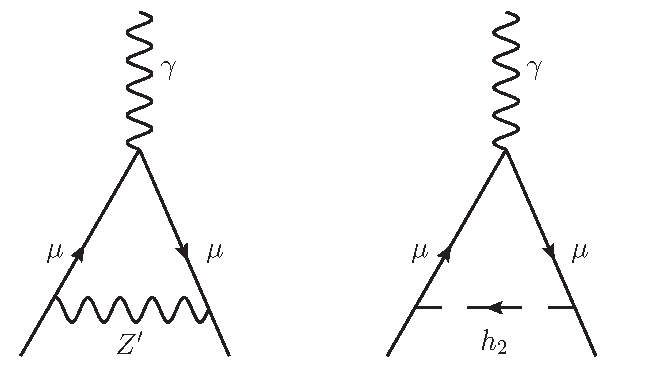
\includegraphics[scale=0.75]{/BLSM/g-2.pdf}
	\caption{One-loop diagrams contributing to $\Delta a_\mu^{\ro{NP}}$ in the B-L-SM.}
	\label{fig:g-2}
\end{figure}	
%%%%%%%%%%%%%%%%%%%%%%%%%

\subsection{Numerical discussion}

For the B-L-SM scan our scanning routine randomly samples parameter space points according to the ranges in Tab.~\ref{tab:scan}.
%
\begin{table}[H]
	\begin{center}
%\begin{ruledtabular}
		\begin{tabular}{ccccc}
			\toprule                     
			$\lambda_{1}$ & $\lambda_{2,3}$ & $g_{\mathrm{B-L}}$ & $g_{\mathrm{YB}}$ & $x~{\mathrm{[TeV]}}$  
			\\       
						\midrule 
			$\left[10^{-2},\; 10^{0.5}
			\right]$ 			    							& $\left[10^{-8},\; 10
			\right]$ 			    							& $\left[10^{-8},\; 10
			\right]$		& $\left[10^{-8},\; 10
			\right]$	&	$\left[0.5,\; 20.5
			\right]$ 	\\
			\bottomrule
		\end{tabular}  
		\caption{Parameter scan ranges used in our analysis. Note that the value of $\lambda_1$ is mostly constrained by the tree-level Higgs boson mass given in Eq.~\eqref{eq:simplify}. 
		}
		\label{tab:scan}
%\end{ruledtabular}
	\end{center}
\end{table}
%  
% { \color{gray} Keeping the remaining free parameters of the model to be in agreement with the Standard Model. } 
%
%The refereed checks applied were sequential and begin with the "zero-th" check where our spectrum generator \texttt{SPheno}, promptly rejects any scenario with tachyonic scalar masses and un-renormalizable quantities.  
%
%\texttt{SPheno} is a particle spectrum generator code written in Fortran 90. It's emphasis on easy generalisability and speed made it a natural part of our numerical analysis. It takes information about our models Lagrangian, such as fields, charges and fundamental symmetries, and creates a executable file capable of quickly generating a spectrum file with all details regarding mass, decay and flavour observables information in the standardized SUSY Les-Houches accord format. All generated spectrums are processed and stored. 
%
%This Lagrangian information is fed to \texttt{SPheno} also in standardized format automatically generated by a Mathematica packaged designed for such purposes called \texttt{SARAH}.  
%
%All inputs and outputs from \texttt{SPheno} are written in the format of a SUSY Les Houches Accord (SLHA) \cite{Skands:2003cj}. 
%
%All points that complete a "zero-th" layer, have all their information regarding two and three body decays, in particular to the Higgs bosons, passed along to another set Fortran 90 packages called \texttt{HiggsBounds} and \texttt{HiggsSignals}. These test experimental detection limits for the new scalars and verify if we have a "SM" like Higgs to account for the detected boson. 
% 
%After this is completed tabular files with all information collected from all programs is saved for later use.
%
%The presence of new bosons in the theory can lead to large deviations in EW precision observables. 

\subsubsection{Electroweak precision observables}

Typically, the most stringent constraints of the scalar sector emerge from the oblique $S,T,U$ parameters, which are also calculated by \texttt{SPheno}. 
%
This conecept was first introduced by Peskin and T. Takeuchi in Ref\,\cite{Peskin1992}.
%
Current precision measurements provide the allowed regions,
%
\begin{equation}
	S = 0.02 \pm 0.10\,, \qquad T = 0.07 \pm 0.12\,, \qquad U = 0.00 \pm 0.09
	\label{eq:oblique}
\end{equation}

%
where $S$-$T$ are $92\%$ correlated, while $S$-$U$ and $T$-$U$ are $-66\%$ and $-86\%$ anti-correlated, respectively.
%
We compare our results with the EW fit in Eq.~\eqref{eq:oblique} and require consistency with the best fit point within a $95\%$ C.L.~ellipsoid (see Ref.~\cite{Costa:2014qga} for further details about this method). %
%
In short we require that the contributions coming from new physics respect the EW precision tests within a 95\% C.L. ellipsoid by imposing, 
%
\begin{equation}
\Delta \chi \equiv \sum_{ij}  \left(  \Delta \mathcal{O}_{i}^{NP} - \mathcal{O}_{i}^{(0)} \right) [ ( \sigma^2 )^{-1} ]_{ij}  \left(  \mathcal{O}_{j}^{NP} - \mathcal{O}_{j}^{(0)}  \right) < 7.815    
\end{equation}
%
Where $\Delta \mathcal{O}_i^{NP} \equiv \mathcal{O}_i - \mathcal{O}^{SM} \rightarrow (\Delta S , \Delta T , \Delta U )$ being that, $\mathcal{O}_i^{(0)}$ is the deviation generated by the Higgs doulbet in the SM if his mass is 125.09. And where the covariance matrix expressed in terms of correlation matrix and started deviations can be seen in, 
\begin{equation}
[ \sigma^2 ]^{-1} \equiv \begin{pmatrix}
867.49 & −904.30 & -360.66\\
−904.30 & 1154.65 & 584.55 \\
−360.66 & 584.55 &  455.19
\end{pmatrix}  
\end{equation}
These values are seen in Ref\,\cite{Baak_2012}. 

We show in Fig.~\ref{fig:STU} our results in the $ST$ (left) and $TU$ (right) planes where black points are consistent with EW precision observables at $95\%$ C.L.~whereas grey ones lie outside the corresponding ellipsoid of the best fit point and, thus, the first points to be excluded in our analysis. 
%%%%%%%%%%%%%%%%%%%%%%%%%
\begin{figure}[H]
	\centering
	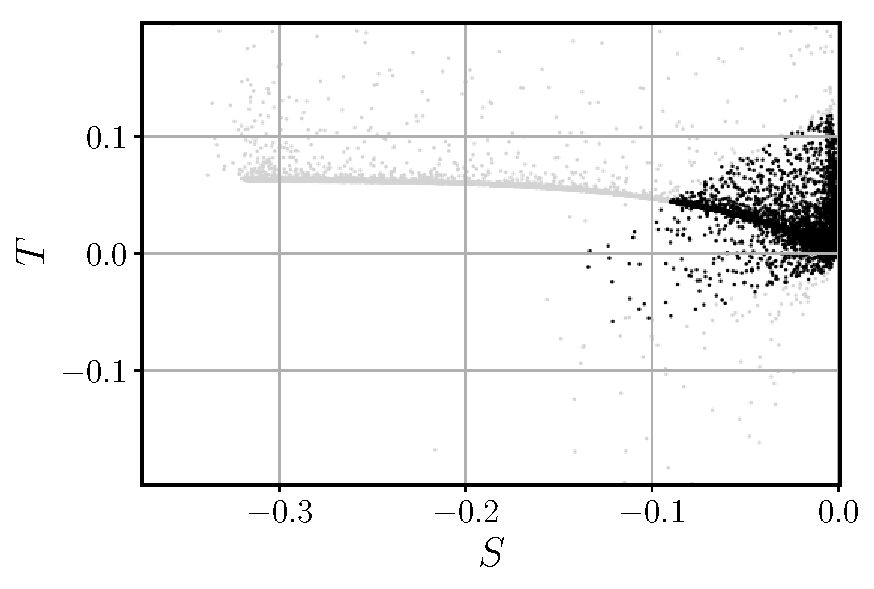
\includegraphics[scale=0.45]{/BLSM/ST.pdf}
	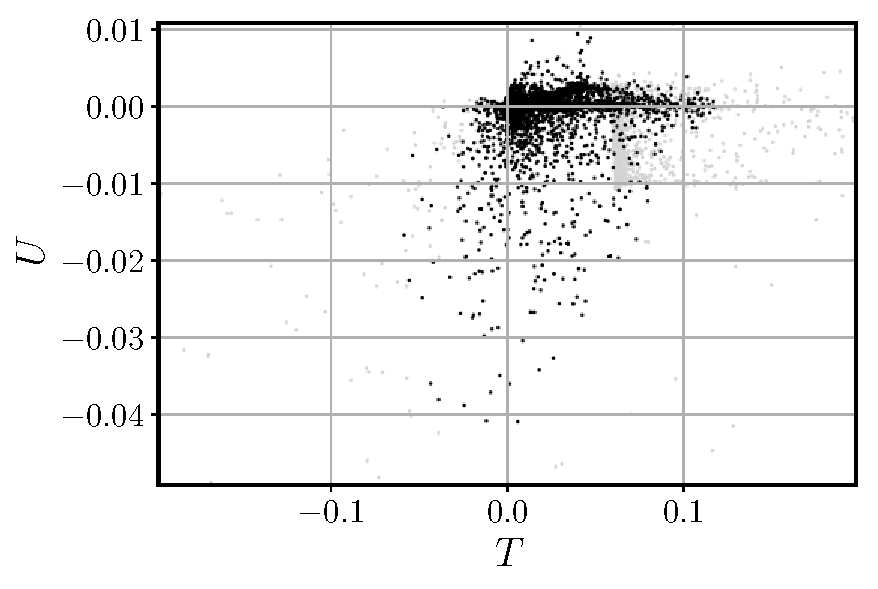
\includegraphics[scale=0.45]{/BLSM/TU.pdf}
	\caption{Scatter plots for EW precision observables showing the $ST$ (left) and $TU$ (right) planes. Accepted points lying within a $95\%$ C.L.~ellipsoid of the best fit point are represented in black whereas grey points are excluded.}
	\label{fig:STU}
\end{figure}	
%%%%%%%%%%%%%%%%%%%%%%%%%

%The B-L-SM predicts a new visible scalar, which we denote as $h_2$, in addition to a SM-like $125~\ro{GeV}$ Higgs boson, $h_1$. 

\subsubsection{Higgs Constraints}

As stated before, we confront the surviving scenarios, black points in Fig.~\ref{fig:STU}, with collider bounds. 
%
In particular the $95\%$ Confidance Level (C.L.) exclusion limits on a new scalar particle and check for consistency with the observed Higgs boson at $3 \sigma$. 
%
These Bounds are checked by \texttt{HiggsBounds/HiggsSignals},  which  is are a set of packages that test the theoretical predictions of our Model from against the exclusion bounds that have been set from Higgs searches at the LHC, LEP and the Tevatron. 
%
We have accepted points whose fit to the data replicates the observed signal at $95\%$ C.L.~while the measured value for its mass, $m_{h_1} = 125.10 \pm 0.14~\textrm{GeV}$ \cite{Tanabashi:2018oca}. 
%
The information required for this check is the the number of neutral and charged Higgs bosons and the information generated by the \texttt{SPheno} output in the format of a SUSY Les Houches Accord (SLHA) \cite{Skands:2003cj} file.
%
Specifically, \texttt{SPheno} provides scalar masses, total decay widths, Higgs decay branching ratios as well as the SM-normalized effective Higgs couplings to fermions and bosons squared (that are needed for analysis of the Higgs boson production cross sections). 
%
For details about this calculation, see Ref.~\cite{Bechtle:2013wla}.

The basic value calculated by \texttt{HiggsSignals} is the signal strength modifier $\mu_{x}$ which parametrizes the signal rate of a particular final state $x$ normalized to the SM expectation trougha a peak-centered $\chi^2$ statistical method.

The combined implementation of \texttt{HiggsBounds/HiggsSignals}, looks at the properties of the discovered Higgs and searches for additional Higgs states, which are then either excluded or allowed in the particle spectra of our model. 

%A  sister  computer  code  ofHiggsBoundsisHiggsSignals,  which  can  be  easily  im-plemented  in  the  exclusion  of  parameter  points.   The  computer  codeHiggsSignalsis,therefore,  a  natural  extension  ofHiggsBoundssince  both  take  as  input  the  number  ofneutral Higgs bosons, scalar masses, cross sections, branching ratios, among other physicalquantities.   The  basic  experimental  value  thatHiggsSignalsuses  is  thesignal  strengthmodifierμxx, which parametrizes the signal rate of a particular final statexx, normalizedto the SM expectation.  Finally,HiggsSignalsimplements the peak-centeredχ2method11There could be a compensation coming from the values of the VEVs.36
%to determine quantitatively to what degree the data and the predicted theory of the modelare compatible.  The combined implementation ofHiggsBounds/HiggsSignalslooks atthe properties of the discovered Higgs and searches for additional Higgs states, which arethen either excluded or allowed in the particle spectra of our model.  In our implementationof the 3HDM, we have found that all the points that passHiggsBoundsare extremely likelyto passHiggsSignalsas well due to the alignment limit imp

%For the latter, we have accepted points whose fit to the data replicates the observed signal at $95\%$ C.L.~while the measured value for its mass, $m_{h_1} = 125.10 \pm 0.14~\textrm{GeV}$ \cite{Tanabashi:2018oca}, is reproduced within a $3\sigma$ uncertainty. 
%The required input data for \texttt{HiggsBounds/HiggsSignals} are generated by the \texttt{SPheno} output in the format of a SUSY Les Houches Accord (SLHA) \cite{Skands:2003cj} file.
%
%In particular, it provides scalar masses, total decay widths, Higgs decay branching ratios as well as the SM-normalized effective Higgs couplings to fermions and bosons squared (that are needed for analysis of the Higgs boson production cross sections). For details about this calculation, see Ref.~\cite{Bechtle:2013wla}.
%
%On a third layer of phenomenological tests we have studied the viability of the surviving scenarios from the perspective of direct collider searches for a new $Z^\prime$ gauge boson. We have used \texttt{MadGraph5\_aMC@NLO 2.6.2} \cite{Alwall:2014hca} to compute the $Z^\prime$ Drell-Yan production cross section and subsequent decay into the first and second-generation leptons, i.e.~$ \sigma \left( pp \to Z^\prime \right) \times B \left( Z^\prime \to \ell \ell\right)$ with $\ell = e,\; \mu$, and then compared our results to the most recent ATLAS exclusion bounds from the LHC runs at the center-of-mass energy $\sqrt{s} = 13~\textrm{TeV}$ \cite{Aaboud:2017buh}. The \texttt{SPheno} SLHA output files were used as parameter cards for \texttt{MadGraph5\_aMC@NLO}, where the information required to calculate $ \sigma\left(pp \to Z^\prime\right) \times B\left(Z^\prime \to \ell \ell\right()$, such as the $Z^\prime$ boson mass, its total width and decay branching ratios into lepton pairs, is provided. 
%
\subsubsection{$Z^\prime$ Constraints}

From here we move onto the third layer of phenomenological tests we look at the viability of the surviving points from the perspective of direct collider searches for a new $Z^\prime$ gauge boson at the most recent collider experiments.
%
We have used \texttt{MadGraph5\_aMC@NLO 2.6.2} \cite{Alwall:2014hca}, with it we compute the $Z^\prime$ Drell-Yan production cross section and subsequent decay into the first and second-generation leptons, i.e.~$ \sigma \left( pp \to Z^\prime \right) \times B \left( Z^\prime \to \ell \ell\right)$ with $\ell = e,\; \mu$, and then compared our results to the most recent ATLAS exclusion bounds from the LHC runs at the center-of-mass energy $\sqrt{s} = 13~\textrm{TeV}$ \cite{Aaboud:2017buh}.

The \texttt{SPheno} SLHA output files were used as parameter cards for \texttt{MadGraph5\_aMC@NLO}, where the information required to calculate $ \sigma\left(pp \to Z^\prime\right) \times B\left(Z^\prime \to \ell \ell\right()$, such as the $Z^\prime$ boson mass, its total width and decay branching ratios into lepton pairs, is provided. 
%
% In this article, we study whether the muon anomalous magnetic moment can be totally or partially explained in the model under consideration and all scenarios with an excessive contribution to $\Delta a_\mu^{\textrm{NP}}$ larger than the upper $2 \sigma$ bound in Eq.~(\ref{g-2}) were rejected.
%
%\subsubsection{Discussion of numerical results}
%\label{sec:discuss}
%
%
Let us now discuss the phenomenological properties of the B-L-SM model. First, we focus on the current collider constraints and study their impact on both the scalar and gauge sectors.
%%%%%%%%%%%%%%%%%%%%%%%%%
\begin{figure}[H]
	\centering
	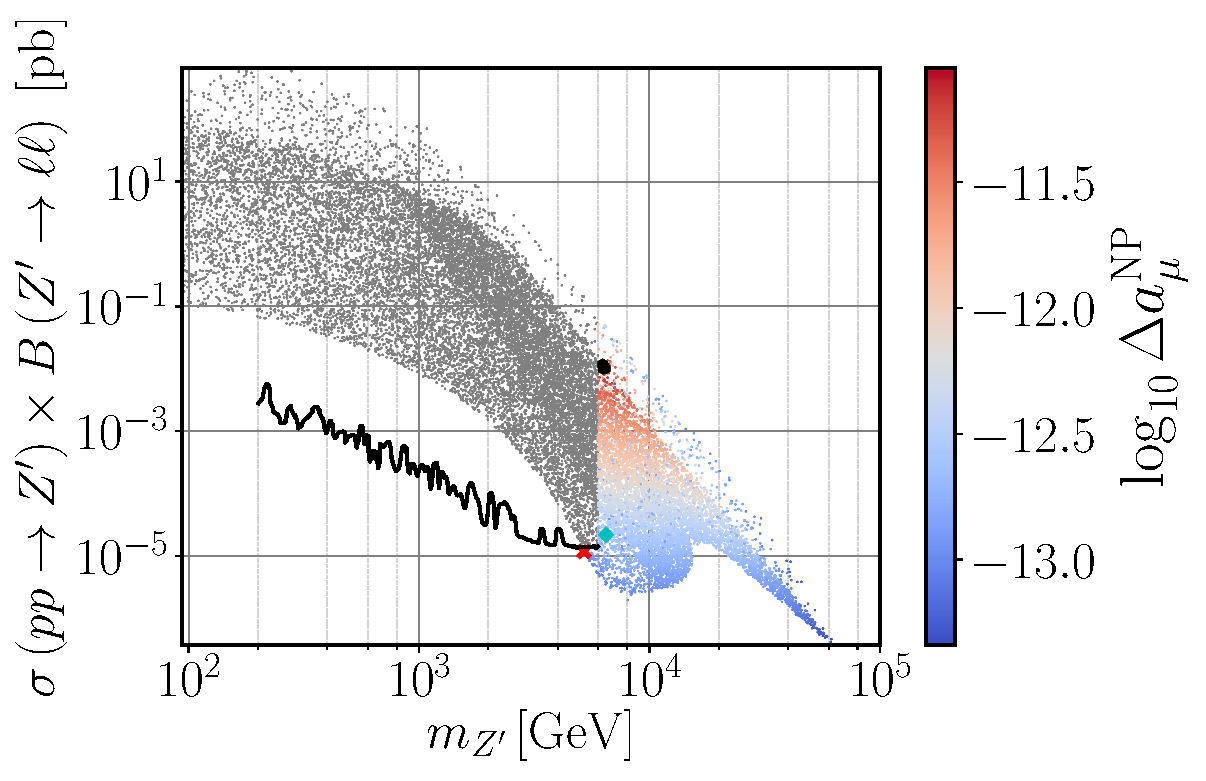
\includegraphics[scale=0.37]{/BLSM/mZp_Xsec_Amu.pdf}
	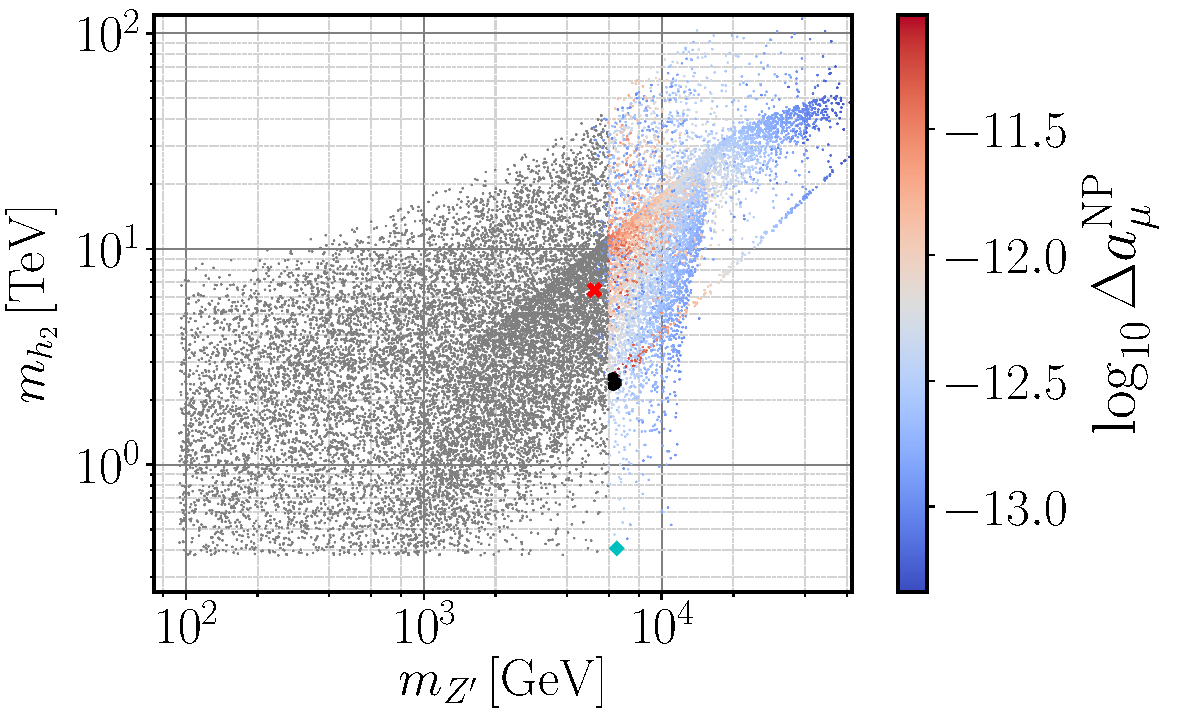
\includegraphics[scale=0.37]{/BLSM/mZp_Mhp_Amu.pdf}
	\caption{Scatter plots showing the $Z^\prime$ Drell-Yan production cross section times the decay branching ratio into a pair of electrons and muons (left panel) and the new scalar mass $m_{h_2}$ (right panel) as functions of $m_{Z^\prime}$ and the new physics (NP) contributions to the muon $\Delta a_\mu$ anomaly. Coloured points have survived all theoretical and experimental constraints while grey points are excluded by direct $Z^\prime$ searches at the LHC. The region between the two dashed lines represents the current ATLAS expected limit on the production cross section times branching ratio into a pair of leptons at $95\%$ C.L.~and is taken from the plot in Fig.~4 of Ref.~\cite{Aaboud:2017buh}. The four highlighted points in both panels denote the benchmark scenarios described in detail in Tab.~\ref{tab:bench}.}
	\label{fig:Plots1}
\end{figure}	
%%%%%%%%%%%%%%%%%%%%%%%%%

We show in Fig.~\ref{fig:Plots1} the scenarios generated in our parameter space scan (see Tab.~\ref{tab:scan}) that have passed all theoretical constraints such as boundedness from below, unitarity and EW precision tests, and experimental restrictions, such as the compatability with the SM Higgs data and where a new visible scalar $h_2$ is unconstrained by the direct collider searches.
%
On the left panel, we show the $Z^\prime$ production cross section times its branching ratio to the first- and second-generation leptons, $\sigma B \equiv \sigma \left( pp \to Z^\prime \right) \times B \left( Z^\prime \to \ell \ell \right) $ with $\ell = e,\mu$, as a function of the new vector boson mass and the new physics contribution to the muon anomalous magnetic moment $\Delta a^{\textrm{NP}}_\mu$ (colour scale). 
%
On the right panel, we show the new scalar mass as a function of the $Z^\prime$ Mass. 
%
All points above the red dashed line are excluded at $95\%$ C.L.~by the upper expected limit on $Z^\prime$ direct searches at the LHC by the ATLAS experiment and are represented in grey shades. 
%
Darker shades denote \textit{would-be-scenarios} with larger values of $\Delta a^{\textrm{NP}}_\mu$ while the smaller contributions to the muon $\left(g-2\right)_\mu / 2$ anomaly are represented with the lighter shades. 
%
The region between the two dashed lines corresponds to the $Z^\prime$ ATLAS limit with a $2\sigma$ uncertainty represented by the yellow band in Fig.~4 of \cite{Aaboud:2017buh}.
%
Provided that the observed limit by the ATLAS detector lies within this region we have taken a conservative approach and accepted all points whose $\sigma B$ value lies below the red dashed line (upper limit) in Fig.~\ref{fig:Plots1}.
%
The blue dashed line, which corresponds to the stricter $2 \sigma$ lower bound, is only shown for completeness of information. The red cross in our figures signals the lightest $Z^\prime$ found in our scan which we regard as a possible early-discovery (or early-exclusion) benchmark point in the forthcoming LHC runs. Such a benchmark point is shown in the first line of Tab.~\ref{tab:bench}.
%
On the right panel, we notice that the new scalar bosons can become as light as $380 - 400~\textrm{GeV}$, but with $Z^\prime$ masses in the range of $5 - 9~\textrm{TeV}$. We highlight with a magenta diamond the benchmark point with the lightest $Z^\prime$ boson within this range. 
%
This point is shown in the second line of Tab.~\ref{tab:bench}.
%
\begin{table}[H]
	\begin{center}
	%\resizebox{\columnwidth}{!}{%
%\begin{ruledtabular}
		\begin{tabular}{cccccccc}
			% \toprule                     
			$m_{Z^\prime}$ & $m_{h_2}$ &  $x$ & $ \log_{10} \Delta a_\mu^{\ro{NP}}$ & $\sigma B$ & $\theta_W^\prime$ & $\alpha_h$ & $g_{\ro{B-L}} \simeq g^{\ell \ell Z^\prime}$ \vspace{1mm}
			\\
			\hline \vspace{-2mm} \\ 
			%%%%%%%%%%
			$3.13$ 			    							& $3.72$ 			    				& $15.7$		& $-12.1$	&	$2.22\times 10^{-4}$ &	$\approx 0$ &	$5.67 \times 10^{-5}$ &	$0.0976$\vspace{1mm} 	\\
			%%%%%%%%%%
			$5.37$ 			    							& $0.396$ 			    				& $9.10$		& $-11.7$	&	$4.23 \times 10^{-5}$ &	$2.55 \times 10^{-7}$ &	$9.44 \times 10^{-7}$ &	$0.302$\vspace{1mm}  	\\
			%%%%%%%%%%
			$7.35$ 			    							& $1.49$ 			    				& $0.321$		& $-8.75$	&	$0.0115$ &	$1.83 \times 10^{-7}$ &	$1.20 \times 10^{-6}$ &	$3.15$\vspace{1mm}  	\\
			%%%%%%%%%%
			$5.91$ 			    							& $1.32$ 			    				& $0.335$		& $-8.78$	&	$0.0285$ &	$1.30 \times 10^{-4}$ &	$1.04 \times 10^{-5} $ &	$2.94$\vspace{1mm}  	\\
%			\bottomrule
		\end{tabular}
%		\end{ruledtabular}
		%}
		\caption{A selection of four benchmark points represented in Figs.~\ref{fig:Plots1}, \ref{fig:Plots4} to \ref{fig:Plots2}. The $m_{Z^\prime}$, $m_{h_2}$ and $x$ parameters are given in TeV. The first line represents a point with light $h_2$ while the second line shows the lightest allowed $Z^\prime$ boson found in our scan. The last two lines show two points that reproduce the observed value of the muon $(g-2)$ within $1\sigma$ uncertainty.}
		\label{tab:bench}
	\end{center}
\end{table}
% 
\subsubsection{Implications of direct $Z^\prime$ searches at the LHC for the $\left(g-2\right)_\mu$ anomaly}

Looking again to Fig.~\ref{fig:Plots1} (left panel), we see that there is a thin dark-red stripe where $\Delta a^{\ro{NP}}_\mu$ explains the observed anomaly shown in Eq.~(\ref{g-2}) for a range of $m_{Z^\prime}$ boson masses approximately between $5~\ro{TeV}$ and $20~\ro{TeV}$. This region is particularly interesting as it can be partially probed by the forthcoming LHC runs or at future colliders. If a $Z^\prime$ boson discovery remains elusive for such a mass range, it can exclude a possibility of explaining the muon $\left(g-2\right)_\mu$ anomaly in the context of the B-L-SM. It is also worth noticing that such preferred $\Delta a^{\ro{NP}}_\mu$ values represent a small island in the right plot of Fig.~\ref{fig:Plots1} where the new scalar boson mass is restricted to the range of $1~\ro{TeV} < m_{h_2} < 4~\ro{TeV}$.


Since the couplings of a new scalar $h_2$ to the SM fermions are suppressed by a factor of $\sin \alpha_h$, which we find to be always smaller than $0.08$ as can be seen in the bottom panel of Fig.~\ref{fig:Plots4}, the right diagram in Fig.~\ref{fig:g-2}, which scales as $\Delta a_\mu^{h_2} \propto {m_\mu^2}/{m_{h_2}^2}\left(y_\mu \sin \alpha_h\right)^2$ with $\sin^2 \alpha_h < 0.0064$ and $y_\mu = Y_e^{22}$, providing sub-leading contributions to $\Delta a_{\mu}$. Furthermore, as we show in the top-left panel of Fig.~\ref{fig:Plots4} the new scalar boson mass, which we have found to satisfy $m_{h_2} \gtrsim 380~\ro{GeV}$, is not light enough to compensate the smallness of the scalar mixing angle. Conversely,  the new $Z^\prime$ boson can have sizeable couplings to fermions via gauge interactions proportional to $g_{\rm B-L}$. Therefore, the left diagram in Fig.~\ref{fig:g-2} provides the leading contribution to the $\left(g-2\right)_\mu$ in the model under consideration.
%%%%%%%%%%%%%%%%%%%%%%%%%
\begin{figure}[!htb]
	\centering
	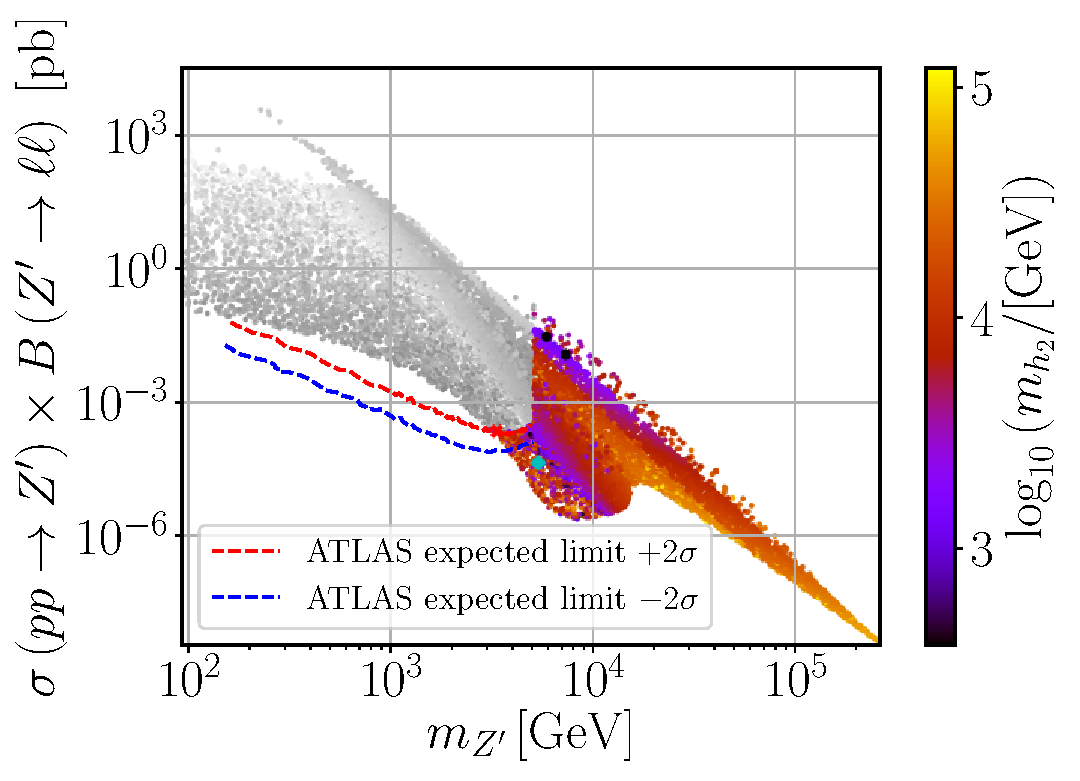
\includegraphics[scale=0.37]{/BLSM/mZp_Xsec_mh2.pdf}
	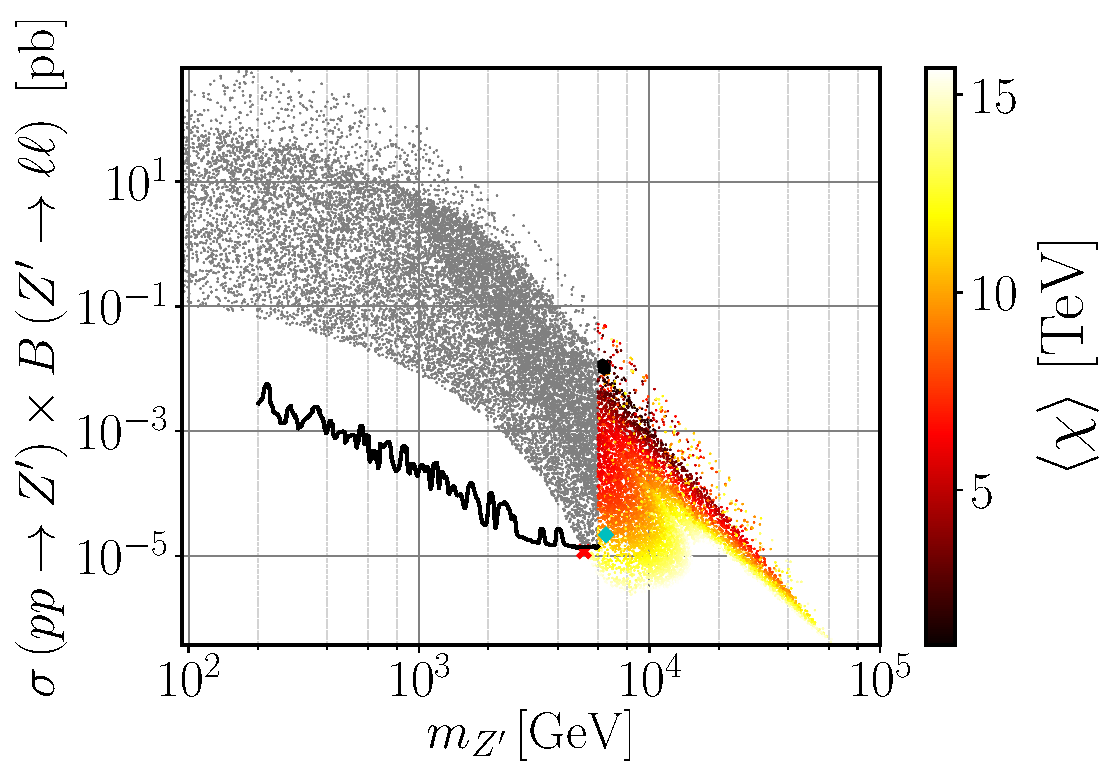
\includegraphics[scale=0.37]{/BLSM/mZp_Xsec_VEV.pdf}
	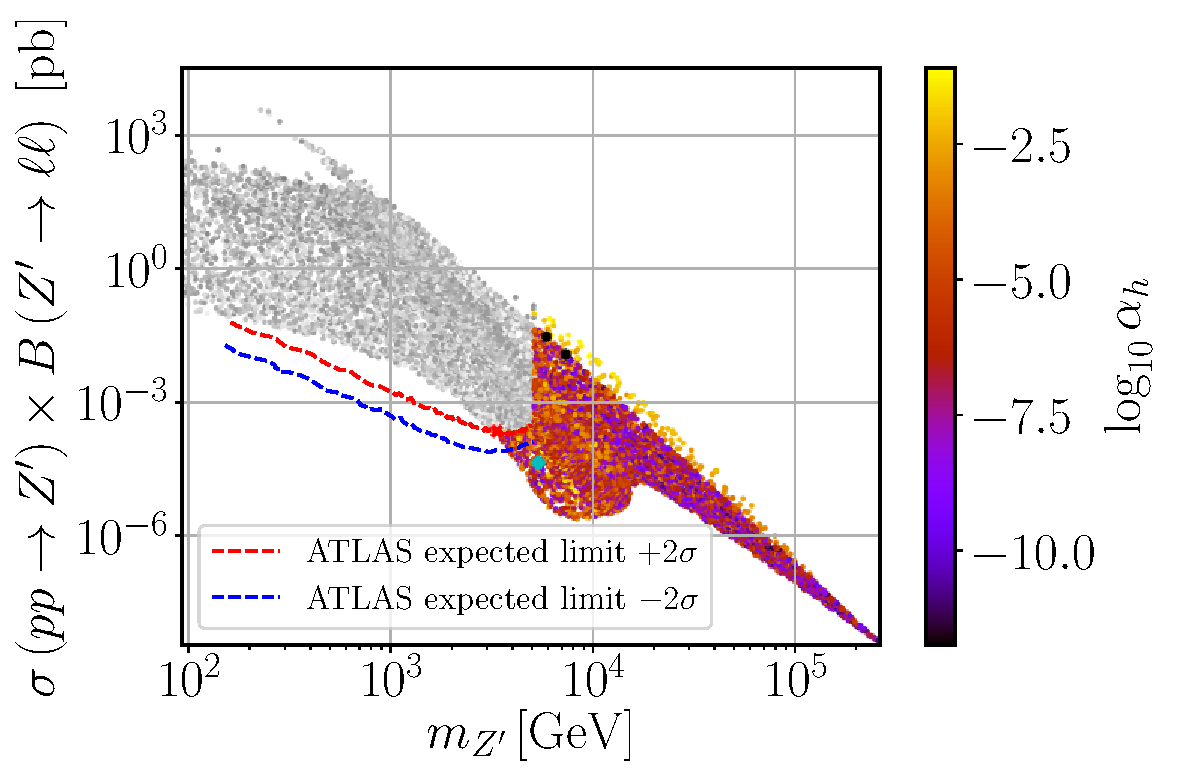
\includegraphics[scale=0.37]{/BLSM/mZp_Xsec_alpha.pdf}	
	\caption{Scatter plots showing the $Z^\prime$ Drell-Yan production cross section times the decay branching ratio into a pair of electrons and muons in terms of the $m_{Z^\prime}$ boson mass. The colour gradation represents the new scalar mass (top-left), the ratio between the EW- and $\U{B-L}$-breaking VEVs (top-right) and the scalar mixing angle (bottom). The grey points are excluded by direct $Z^\prime$ searches at the LHC. The four benchmark points in Tab.~\ref{tab:bench} are represented by the black dots (last two rows), cyan diamond (first row) and red cross (second row).}
	\label{fig:Plots4}
\end{figure}	
%%%%%%%%%%%%%%%%%%%%%%%%%
In particular, $\Delta a_\mu^{Z^\prime}$ is given by \cite{Freitas:2014pua}
\begin{equation}
\Delta a_\mu^{Z^\prime} = \tfrac{1}{12 \pi^2} \tfrac{m_{\mu}^2}{m_{Z^\prime}^2} \(3 g_{\rm L}^{\mu \mu Z^\prime} g_{\rm R}^{\mu \mu Z^\prime} - {g_{\rm L}^{\mu \mu Z^\prime}}^2 - {g_{\rm R}^{\mu \mu Z^\prime}}^2 \)
\label{eq:ZpContribution}
\end{equation}
where the left- and right-chiral projections of the charged lepton couplings to the $Z^\prime$ boson, $g_{\rm L}^{\ell \ell Z^\prime}$ and $g_{\rm R}^{\ell \ell Z^\prime}$, respectively, can be approximated as follows
\begin{equation}
\begin{aligned}
    g_{\rm L}^{\ell \ell Z^\prime} &\simeq g_{\rm B-L} + \tfrac{1}{32} \(\tfrac{v}{x}\)^2 \tfrac{g_{\rm YB}}{g_{\rm B-L}} \[g_{\rm Y}^2 - g^2 + 2 g_{\rm Y}g_{\rm YB}\]\,,
    \\
    g_{\rm R}^{\ell \ell Z^\prime} &\simeq g_{\rm B-L} + \tfrac{1}{16} \(\tfrac{v}{x}\)^2 \tfrac{g_{\rm YB}}{g_{\rm B-L}} \[g_{\rm Y}^2 + g_{\rm Y}g_{\rm YB}\]\,,
\end{aligned}\label{eq:gllZ}
\end{equation}
to second order in $v/x$-expansion. If $v/x \ll 1$, corresponding to the darker shades of the color scale in the top-right panel of Fig.~\ref{fig:Plots4}, we can further approximate
%
\begin{equation}
    g_{\rm L}^{\ell \ell Z^\prime} \simeq g_{\rm R}^{\ell \ell Z^\prime} \simeq g_{\ro{B-L}}\,,
    \label{eq:gLgR-simp}
\end{equation}
%
such that the muon anomalous magnetic moment gets significantly simplified to
\begin{equation}
\Delta a_\mu^{Z^\prime} \simeq \dfrac{g_{\ro{B-L}}^2}{12 \pi^2} \dfrac{m_{\mu}^2}{m_{Z^\prime}^2}\,.
\label{eq:amu-simple}
\end{equation}
%
Similarly, for the yellow band in the bottom of Fig.~\ref{fig:Plots3}, which corresponds to the region where $\Delta a_{\mu}^{\rm NP}$ is maximized (see top-left panel of Fig.~\ref{fig:Plots1}), a large value of the $\U{B-L}$ gauge coupling also allows one to simplify Eq.~\eqref{eq:ZpContribution} reducing it to the form of Eq.~\eqref{eq:amu-simple}. This is in fact what we have observed and, for the yellow band region, we see in the bottom panel of Fig.~\ref{fig:Plots3} that $g_{\ro{B-L}} \simeq 3$. A sizeable value of $g_{\ro{B-L}}$ is indeed what is contributing to the enhancement of $\Delta a_{\mu}^{\rm NP}$, in particular, for the red region in both panels of Fig.~\ref{fig:Plots1}. We show in the third and fourth lines of Tab.~\ref{tab:bench} the two benchmark points that better reproduce the muon anomalous magnetic moment represented by two black dots in
Figs.~\ref{fig:Plots1}, \ref{fig:Plots4} to \ref{fig:Plots2}.
%%%%%%%%%%%%%%%%%%%%%%%%%
\begin{figure}[!htb]
	\centering
	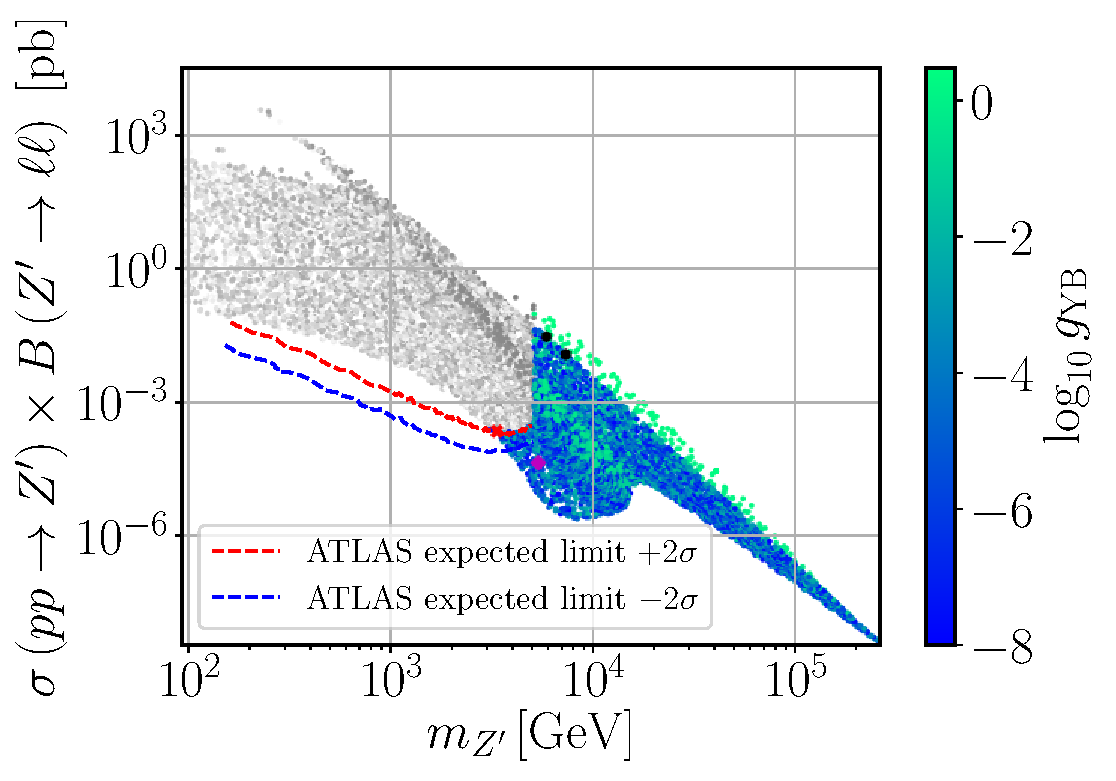
\includegraphics[scale=0.37]{/BLSM/mZp_Xsec_gYB.pdf}
	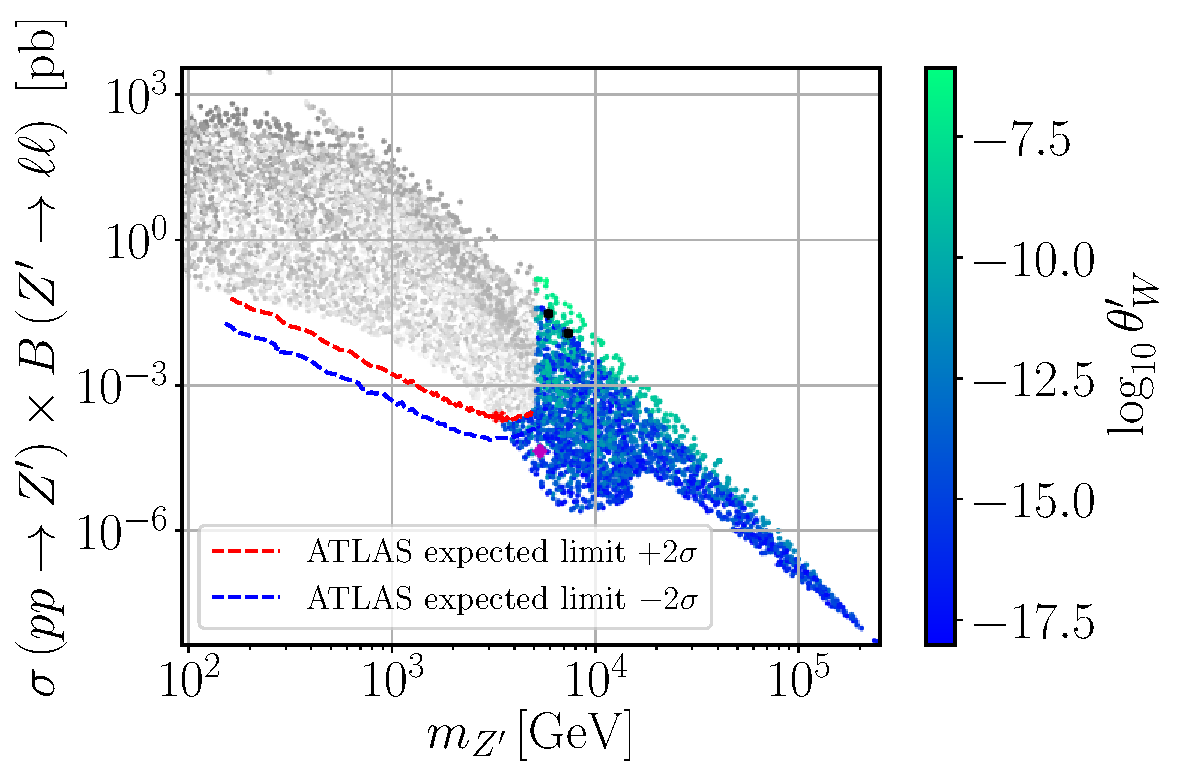
\includegraphics[scale=0.37]{/BLSM/mZp_Xsec_twp.pdf}
	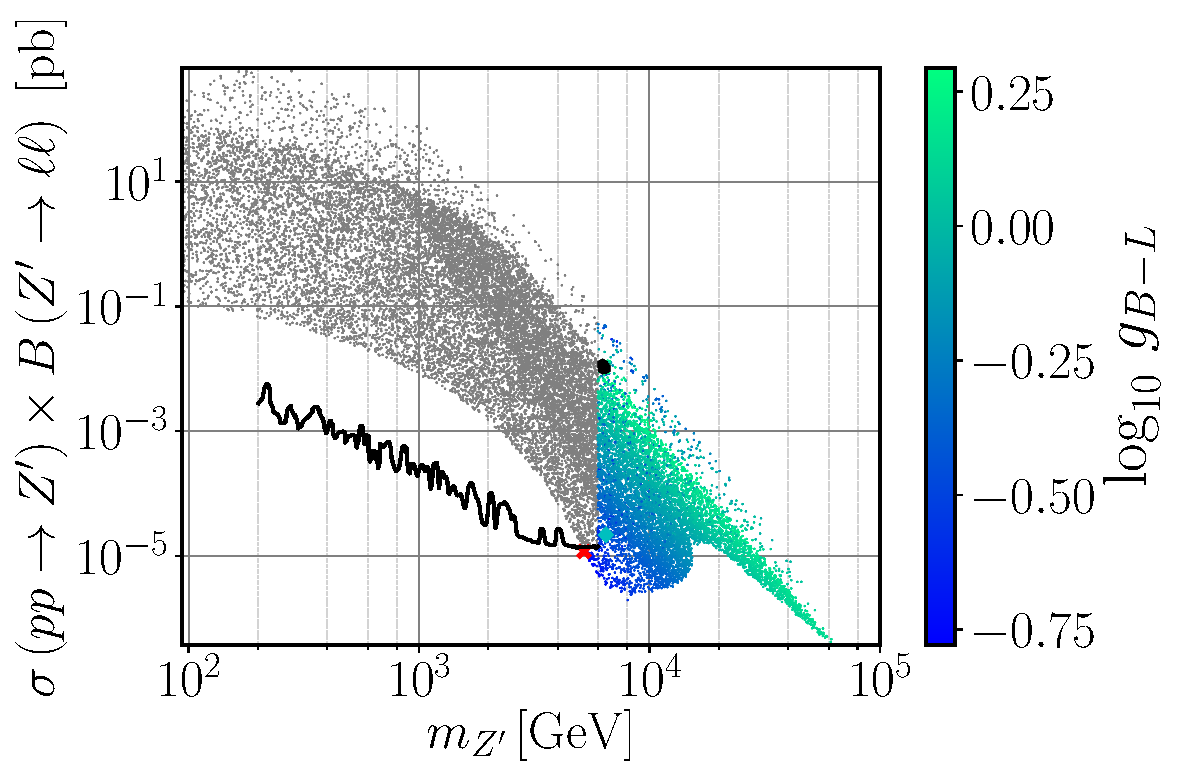
\includegraphics[scale=0.37]{/BLSM/mZp_Xsec_gBL.pdf}	
	\caption{The same as in Fig.~\ref{fig:Plots4} but with the colour scale representing the gauge-mixing parameters $g_{\ro{YB}}$ (top-left), $\theta_{W}^{\prime}$ (top-right), and the $\U{B-L}$ gauge coupling (bottom).}
	\label{fig:Plots3}
\end{figure}	
%%%%%%%%%%%%%%%%%%%%%%%%%

In fact, a close inspection of Fig.~\ref{fig:Plots1} (left panel) and Fig.~\ref{fig:Plots4} (top-right panel) reveals an almost one-to-one correspondence between the colour shades. 
This suggests that $\Delta a_{\mu}^{Z^\prime}$ must somehow be related to the VEV ratio $v/x$. 
To understand this behaviour, let us also look to Fig.~\ref{fig:Plots3} (top-left panel) where we see that the kinetic-mixing gauge coupling $g_{\ro{YB}}$ is typically very small apart from two green bands where it can become of order $\mathcal{O}(1)$.
Interestingly, whenever $g_{\ro{YB}}$ becomes sizeable, $v/x \ll 1$ is realised, which means that Eq.~\eqref{eq:mZ} is indeed a good approximation as was argued above. It is then possible to eliminate $g_{\ro{B-L}}$ from Eq.~\eqref{eq:amu-simple} and rewrite it as
\begin{equation}
    \Delta a_\mu^{Z^\prime} \simeq \dfrac{y_\mu^2}{96 \pi^2} \(\dfrac{v}{x}\)^2 \,,
    \label{eq:amu-vev}
\end{equation}
which explains the observed correlation between both Fig.~\ref{fig:Plots1} (left panel) and Fig.~\ref{fig:Plots4} (top-right panel) and, for instance, the thin red stripe of points is compatible with a full description of the muon $\left(g-2\right)_{\mu}/2$ anomaly. Note that this simple and illuminating relation becomes valid as a consequence of the heavy $Z^\prime$ mass regime, in combination with the smallness of the $\theta_{W}^{\prime}$ mixing angle required by LEP constraints. Indeed, while we have not imposed any strong restriction on the input parameters of our scan (see Tab.~\ref{tab:scan}), Eq.~\eqref{eq:theta-p} necessarily implies that both $g_{\ro{YB}}$ and $v/x$ cannot be simultaneously sizeable in agreement with what is seen in Fig.~\ref{fig:Plots3} (top-left panel) and Fig.~\ref{fig:Plots4} (top-right panel). The values of $\theta_W^\prime$ obtained in our scan are shown in the top-right panel of Fig.~\ref{fig:Plots3}.

For completeness, we show in Fig.~\ref{fig:Plots2} the physical couplings of $Z^\prime$ to muons (top panels) and to $W^\pm$ bosons (bottom panel).
%%%%%%%%%%%%%%%%%%%%%%%%%
\begin{figure}[!htb]
	\centering
	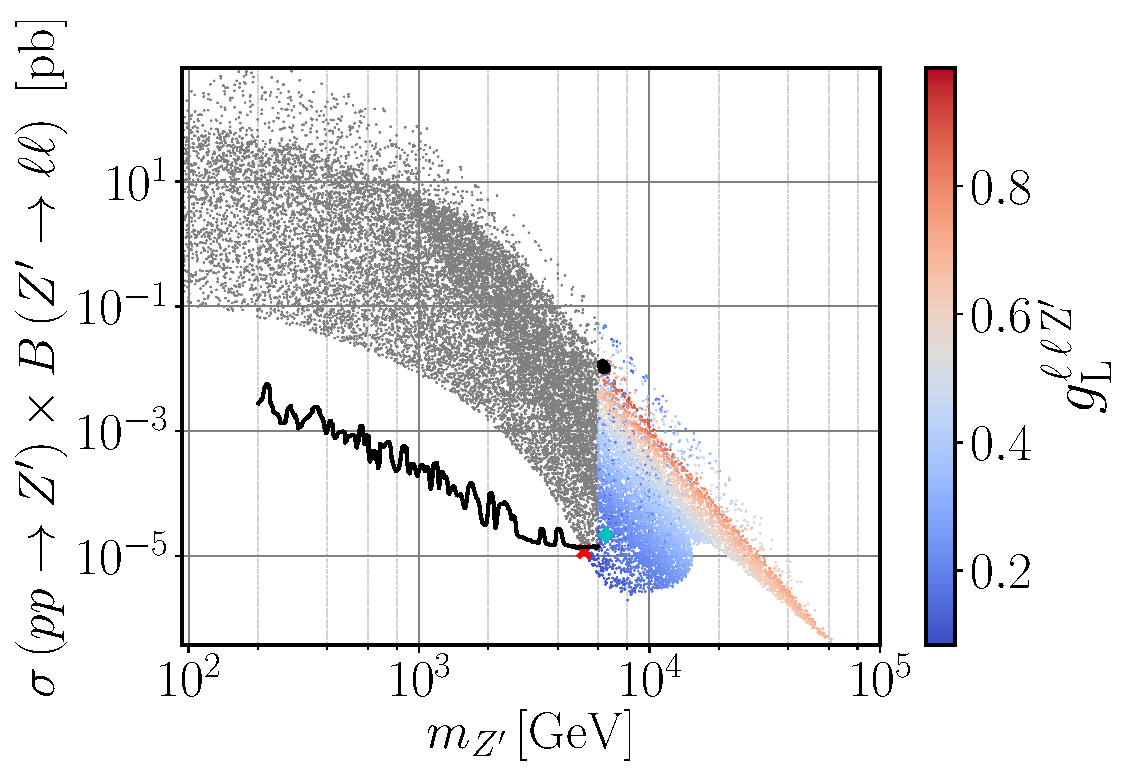
\includegraphics[scale=0.37]{/BLSM/mZp_Xsec_gLmumuZ.pdf}
	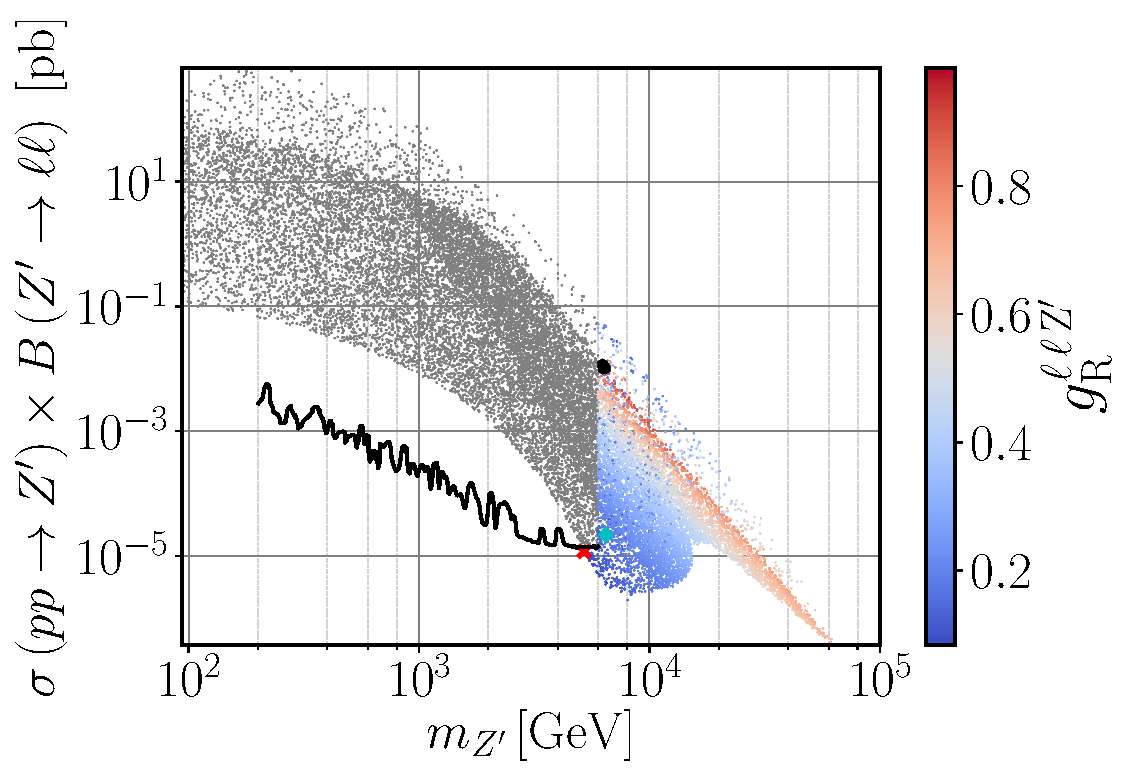
\includegraphics[scale=0.37]{/BLSM/mZp_Xsec_gRmumuZ.pdf}
	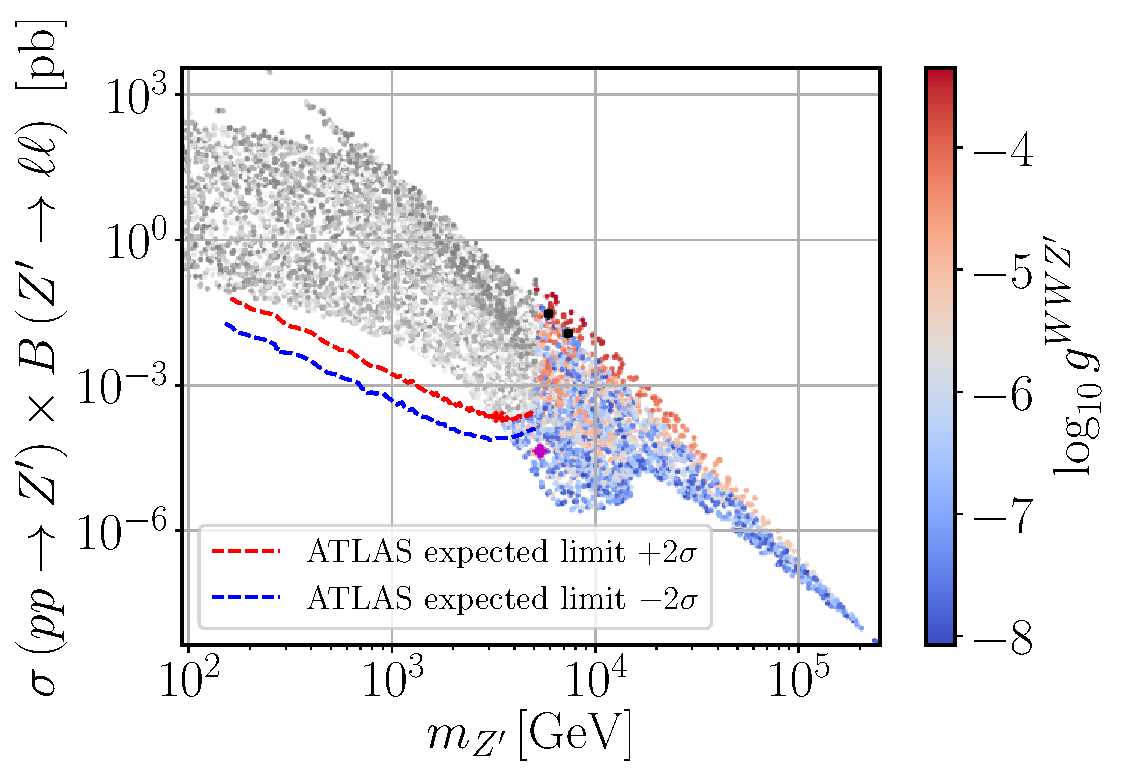
\includegraphics[scale=0.37]{/BLSM/mZp_Xsec_gWWZp.pdf}
	\caption{The same as in Fig.~\ref{fig:Plots4} but with the colour scale representing the coupling of leptons to the $Z^\prime$ (top panels) and the coupling of $W$ bosons to $Z^\prime$.}
	\label{fig:Plots2}
\end{figure}	
%%%%%%%%%%%%%%%%%%%%%%%%%
Note that, for the considered scenarios, the latter can be written as
\begin{equation}
    g^{WWZ^\prime} \simeq \dfrac{1}{16} \dfrac{g_{\ro{YB}}}{g_{\ro{B-L}}} \(\dfrac{v}{x}\)^2\,.
    \label{eq:gWWZp}
\end{equation}
While both $g_{\ro{B-L}}$ and the ratio $v/x$ provide a smooth continuous contribution in the $\sigma B - m_{Z^\prime}$ projection of the parameter space, the observed blurry region in $g^{WWZ^\prime}$ is correlated with the one in the top-left panel of Fig.~\ref{fig:Plots3} as expected from Eq.~\eqref{eq:gWWZp}. On the other hand, the couplings to leptons $g_{\rm L,R}^{\ell \ell Z^\prime}$ exhibit a strong correlation with $g_{\ro{B-L}}$ in Fig.~\ref{fig:Plots3}, in agreement with our discussion above and with Eq.~\eqref{eq:gLgR-simp}.

\subsubsection{Barr-Zee type contributions}
\label{sec:BarrZee}

To conclude our analysis, one should note that the two-loop Barr-Zee type diagrams \cite{Barr:1990vd} are always sub-dominant in our case. To see this, let us consider the four diagrams shown in Fig.~\ref{fig:Barr-Zee}.
%%%%%%%%%%%%%%%%%%%%%%%%%
\begin{figure}[!htb]
	\centering
	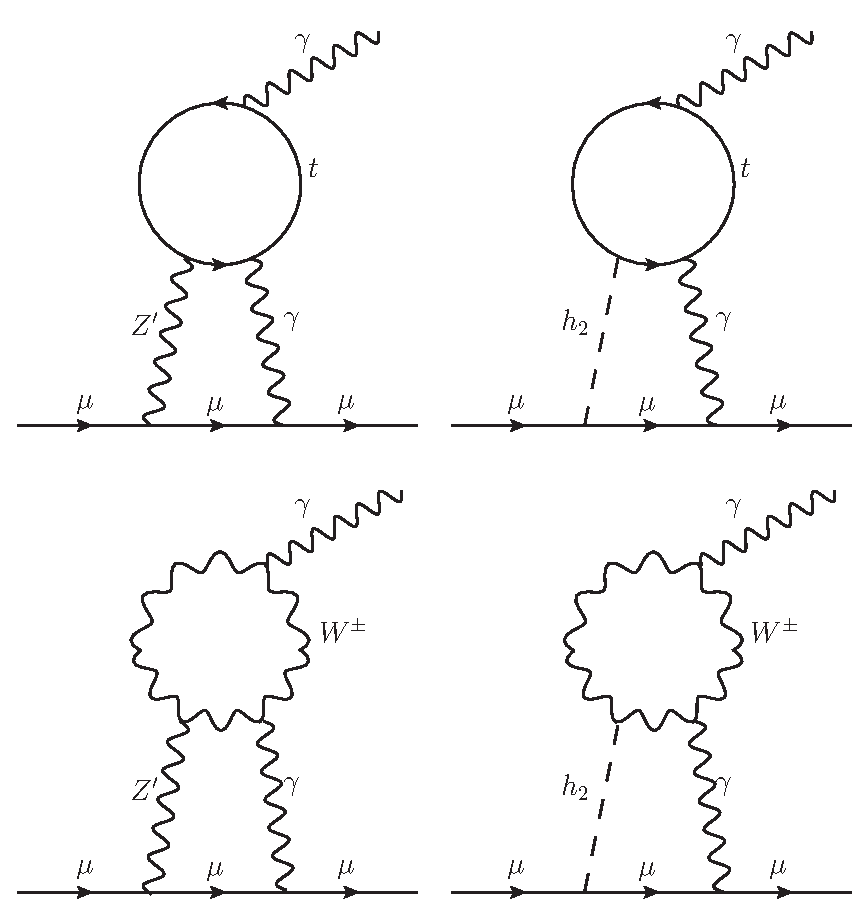
\includegraphics[scale=0.6]{/BLSM/Barr-Zee.pdf}
	\caption{Barr-Zee type two-loop diagrams contributing to $\Delta a_\mu$.}
	\label{fig:Barr-Zee}
\end{figure}	
%%%%%%%%%%%%%%%%%%%%%%%%%
The same reason that suppresses the one-loop $h_2$ contribution in Fig.~\ref{fig:g-2} is also responsible for the suppression of both the top-right and bottom-right diagrams in Fig.~\ref{fig:Barr-Zee} (for details see e.g.~Ref.~\cite{Ilisie:2015tra}). Recall that the coupling of $h_2$ to the SM particles is proportional to the scalar mixing angle $\alpha_h$, which is always small (or very small) as we can see in Fig.~\ref{fig:Plots4}. An analogous effect is present in the diagram involving a $W$-loop, where a vertex proportional to $g^{WWZ^\prime}$ suppresses such a contribution. The only diagram that might play a sizeable role is the top-left one where the couplings of $Z^\prime$ to both muons and top quarks are not negligible.

Let us then estimate the size of the first diagram in Fig.~\ref{fig:Barr-Zee}. This type of diagrams were already calculated in Ref.~\cite{Feng:2009gn} but for the case of a SM $Z$-boson. Since the same topology holds for the considered case of B-L-SM too, 
if we trade $Z$ by the new $Z^\prime$ boson, the contribution to the muon $(g-2)_\mu$ anomaly can be rewritten as
\begin{equation}
    \Delta a_{\mu}^{\gamma Z^\prime} = -\dfrac{g^2 g^2_{\ro{B-L}} m_\mu^2 \tan^2{\theta_W}}{1536 \pi^4} \left( g_{\ro{L}}^{ttZ^\prime} - g_{\ro{R}}^{ttZ^\prime} \right) \ro{T}_7\left( m_{Z^\prime}^2, m_t^2, m_t^2 \right)\,,
    \label{eq:agZ}
\end{equation}
where $T_7$ is a loop integral described in appendix \ref{app:T7}. The parameters $g_{\ro{L,R}}^{ttZ^\prime}$, calculated in \texttt{SARAH}, are the left- and right-chirality projections of the $Z^\prime$ coupling to top-quarks, given by
\begin{equation}
\begin{aligned}
    g_{\ro{L}}^{ttZ^\prime} &= -\dfrac{g_{\ro{B-L}}}{3} \cos{\theta_W^\prime} + \dfrac{g}{2} \cos{\theta_W} \sin{\theta_W^\prime} - \dfrac{g_{\ro{Y}}}{6} \sin{\theta_W} \sin{\theta_W^\prime} - \dfrac{g_{\ro{YB}}}{3} \sin{\theta_W} \sin{\theta_W^\prime}\,,
    \\
    g_{\ro{R}}^{ttZ^\prime} &= -\dfrac{g_{\ro{B-L}}}{3} \cos{\theta_W^\prime} - \dfrac{2 g_{\ro{Y}}}{3} \sin{\theta_W} \sin{\theta_W^\prime} - \dfrac{g_{\ro{YB}}}{3} \sin{\theta_W} \sin{\theta_W^\prime}\,.
\end{aligned}
\end{equation}
The loop integral $\ro{T}_7 \(m_{Z^\prime}^2, m_t^2, m_t^2\)$ was determined in Ref.~\cite{Feng:2009gn} and, in the limit $m_{Z^\prime} \gg m_t$, as we show in Eq.~\eqref{eq:T7-expanded}, it gets simplified to
\begin{equation}
    \ro{T}_7 \(m_{Z^\prime}^2, m_t^2, m_t^2\) \simeq \frac{2}{m_{Z^\prime}^2} \,,
    \label{eq:T7}
\end{equation}
up to a small truncation error (see Appendix~\ref{app:T7} for details). For the parameter space region under consideration the difference $g_{\ro{L}}^{ttZ^\prime} - g_{\ro{R}}^{ttZ^\prime}$ can be cast in a simplified form as follows 
\begin{equation}
    \left(g_{\ro{L}}^{ttZ^\prime} - g_{\ro{R}}^{ttZ^\prime}\right) \simeq \dfrac{\left(g^2+g_{\ro{Y}}^2\right)g_{\ro{YB}}}{32 g_{\ro{B-L}}} \left(\dfrac{v}{x}\right)^2\,.
    \label{eq:gLminusgR}
\end{equation}
Using this result and the approximate value of the loop factor, we can calculate the ratio between 
the two- and one-loop contributions to the muon $(g-2)_{\mu}$,
\begin{equation}
    \dfrac{\Delta a_{\mu}^{\gamma Z^\prime}}{\Delta a_{\mu}^{Z^\prime}} \simeq -\dfrac{g^2 g_{\ro{Y}^2}}{2048 \pi^2} \dfrac{g_{\ro{YB}}}{g_{\ro{B-L}}} \left( \dfrac{v}{x} \right)^2 \ll 1\,,
\end{equation}
which shows that $\Delta a_\mu^{\gamma Z^\prime}$ does indeed play a subdominant role in our analysis and can be safely neglected.


%\section{The B-L-SM Conclusions}
%\label{sec:Conclusions BLSM}

%To summarise, in this work we have performed a detailed phenomenological analysis of the minimal $\U{B-L}$ extension of the Standard Model known as the B-L-SM. 

%In this chapter, we have confronted the model with the most recent experimental bounds from the direct $Z^\prime$ boson and next-to-lightest Higgs state searches at the LHC.
%
%Simultaneously, we have analysed the prospects of the B-L-SM for a consistent explanation of the observed anomaly in the muon anomalous magnetic moment $(g-2)_{\mu}$. 
%
%Done by exploring the B-L-SM potential for the observed $(g-2)_{\mu}$ anomaly in the regions of the model parameter space that are consistent with direct searches and electroweak precision observables.

%As one of the main results of our analysis, we have found phenomenologically consistent parameter space regions that simultaneously fit the exclusion limits from direct $Z^\prime$ searches and can explain the muon $(g-2)_{\mu}$ anomaly. 
%
%We have distinguished four benchmark points for future phenomenological exploration at experiments, the first one with the lightest allowed $Z^\prime$ ($m_{Z^\prime}>3.1$ TeV), the second with the lightest additional scalar boson ($m_{h_2}>400$ GeV), and the other two points that reproduce the muon $(g-2)_{\mu}$ anomaly within $1\sigma$ uncertainty range. 
%
%Besides, we have studied the correlations of the $Z^\prime$ production cross section times the branching ratio into a pair of light leptons versus the physical parameters of the model.
%
%In particular, we have found that the muon $(g-2)_{\mu}$ observable dominated by $Z^\prime$ loop contributions lies within the phenomenologically viable parameter space domain. 
%
%For completeness, we have also estimated the dominant contribution from the Barr-Zee type two-loop corrections and found a relatively small effect.



%\chapter{3HDM}
%\label{ch:3HDM}

\newpage 

\chapter{3HDM}

We have studied the main features and the phenomenological  consistency of a family non-universal Three Higgs Doublet Model or 3HDM with a softly broken $\mathrm{U(1)\times Z_2} $ symmetry group. This broken symmetry will justify the flavour hierarchies in the SM and trough a Branco-Grimus-Lavoura mechanism supress the otherwise expected Flavour Changing Neutral Currents. 

Let us now consider an extended version of the SM, with an enlarged Higgs sector that contains three generations of scalar-doublets. These Higgs will be named $\phi^i$ with $i={1,2,3}$.  In this sector we must enforce the alignment limit to the scalar sector ensuring the physical scalar spectrum accommodates a SM-like Higgs boson with mass of $125.09$ GeV.

%\chapter{Conclusions}
%\label{ch:Conclusions}

\newpage 

\chapter{Conclusions and Future Work}

\newpage

\begin{appendices}

\chapter{The loop integral \texorpdfstring{$\ro{T}_7(x,y,x)$}{} }
\label{app:T7}

In Appendix B of Ref.~\cite{Feng:2009gn}, the exact integral equations for $\ro{T}_7\left(x,y,z\right)$ are provided. 
In our analysis we consider the limit where $x \gg y = z$, with $x = m_{Z^\prime}^2$ and $y = z = m_t^2$, 
where Eq.~\eqref{eq:T7} provides a good approximation up to a truncation error. Here, we show the main steps 
in determining Eq.~\eqref{eq:T7}. The exact form of the loop integral reads as
\begin{equation}
\begin{aligned}
    \ro{T}_7\left(x,y,y\right) =& -\dfrac{1}{x^2} \varphi_0\left(y,y\right) + 2 y \dfrac{\del^3 \Phi(x,y,y)}{\del x \del y^2} + \dfrac{\del^2 \Phi(x,y,y)}{\del x^2} + x \dfrac{\del^3 \Phi(x,y,y)}{\del x^2 \del y} \\
    & + \dfrac{\Phi(x,y,y)}{x^2}
    -\dfrac{1}{x} \dfrac{\del \Phi(x,y,y)}{\del x}
    + \dfrac{\del^2 \Phi(x,y,y)}{\del x \del y} \,,
\end{aligned}    
\label{eq:T7-Integrals}
\end{equation}
with $\varphi_0 (x,y)$ and $\Phi(x,y,z)$ defined in Ref.~\cite{Feng:2009gn}. Let us now expand 
each of the terms for $x \ll y$. While the first term is exact and has the form
\begin{equation}
    -\dfrac{1}{x^2} \varphi_0\left(y,y\right) = -2 \dfrac{y}{x^2} \log^2 y \,,
    \label{eq:expand1}
\end{equation}
the second can be approximated to
\begin{equation}
    2 y \dfrac{\del^3 \Phi(x,y,y)}{\del x \del y^2} \simeq \xi \dfrac{24}{x} = \dfrac{8}{x} ~\textrm{for}~ \xi = \dfrac{1}{3}\,.
    \label{eq:expand2}
\end{equation}
In Eq.~\eqref{eq:expand2}, the $\xi = \tfrac{1}{3}$ factor was introduced in order to compensate for a truncation error. This was obtained by comparing the numerical values of the exact expression and our approximation. The third term can be simplified to
\begin{equation}
    \dfrac{\del^2 \Phi(x,y,y)}{\del x^2} \simeq \dfrac{2}{x} \left( \log y - \log \dfrac{y}{x} \right) + \dfrac{2}{x} \,,
    \label{eq:expand3}
\end{equation}
and the fourth to
\begin{equation}
    x \dfrac{\del^3 \Phi(x,y,y)}{\del x^2 \del y} \simeq -\dfrac{4}{x}\left(\log \dfrac{y}{x} + 1 \right)\,.
    \label{eq:expand4}
\end{equation}
The fifth and the seventh terms read
\begin{equation}
    \dfrac{\Phi(x,y,y)}{x^2}
    -\dfrac{1}{x} \dfrac{\del \Phi(x,y,y)}{\del x} \simeq \dfrac{2}{x} \log \dfrac{1}{x} \,,
    \label{eq:expand5}
\end{equation}
and finally, the sixth terms can be expanded as
\begin{equation}
    \dfrac{\del^2 \Phi(x,y,y)}{\del x \del y} \simeq \dfrac{4}{x}\left(\log \dfrac{y}{x} -1\right)\,.
    \label{eq:expand6}
\end{equation}
Noting that Eq.~\eqref{eq:expand1} is of the order $\tfrac{1}{x^2}$, putting together Eqs.~\eqref{eq:T7-Integrals}, \eqref{eq:expand2}, \eqref{eq:expand3}, \eqref{eq:expand4}, \eqref{eq:expand5}, and \eqref{eq:expand6} we get for the leading $\tfrac{1}{x}$ contributions the following:
\begin{equation}
    \begin{aligned}
    \ro{T}_7\left(x,y,y\right) \simeq& \overbrace{\dfrac{2}{x} \( \log y - \log \dfrac{y}{x} \) + \dfrac{2}{x} \log \dfrac{1}{x}}^{0} \overbrace{-\dfrac{4}{x}\(\log \dfrac{y}{x} + 1 \) +
    \dfrac{4}{x}\(\log \dfrac{y}{x} -1\)}^{-\tfrac{8}{x}} + \dfrac{8}{x} + \dfrac{2}{x} \simeq \dfrac{2}{x}\,.
    \end{aligned}
    \label{eq:T7-expanded}
\end{equation}
\end{appendices}

\newpage

\bibliography{./bib.bib}
\bibliographystyle{ieeetr}

\end{document}
